\documentclass[12pt, oneside]{article}

\setlength{\headheight}{15.71667pt}


\usepackage[spanish]{babel}
\usepackage{apacite}

\addto\captionsspanish{%
  \renewcommand{\tablename}{Tabla}
}

\usepackage[table,xcdraw]{xcolor}

\usepackage[T1]{fontenc}
% \usepackage{uarial}
% \renewcommand{\familydefault}{\sfdefault}

\usepackage{etoolbox}
\patchcmd{\thebibliography}{\section*{\refname}}{}{}{}


\usepackage{url}
\def\UrlBreaks{\do\/\do-}

\usepackage{adjustbox}
\usepackage{graphicx}
\usepackage{tabularx}
\usepackage{svg}
\usepackage{float}
\restylefloat{table}

\usepackage{enumitem}

\usepackage{multicol}

\parskip=12pt 
\parindent=0pt

\usepackage{ragged2e}
\tolerance=1
\emergencystretch=\maxdimen
\hyphenpenalty=10000
\hbadness=10000
\raggedright

\usepackage{textcase}
\usepackage{tocloft}
\makeatletter
\patchcmd{\l@section}{#1}{\MakeTextUppercase{#1}}{}{}
\patchcmd{\l@subsection}{#1}{\MakeTextUppercase{#1}}{}{}
\patchcmd{\l@subsubsection}{#1}{\MakeTextUppercase{#1}}{}{}
\makeatother

\usepackage{titlesec}
\titleformat{\section}{\raggedright\normalfont\normalsize\bfseries\uppercase}{\thesection}{1em}{}
\titleformat{\subsection}{\raggedright\normalfont\normalsize\bfseries\uppercase}{\thesubsection}{1em}{}
\titleformat{\subsubsection}{\raggedright\normalfont\normalsize\bfseries\uppercase}{\thesubsubsection}{1em}{}

\usepackage{geometry}
\geometry {
    letterpaper,
    left = 1in,
    right = 1in,
    bottom = 1in,
    top = 1in
}

% Line break
\newcommand{\skipline}{\par\null\par}

\usepackage{subfig}

\newcommand*{\Universidad}[1]{\def\Uni{#1}}
\newcommand*{\Facultad}[1]{\def\Fac{#1}}
\newcommand*{\Escuela}[1]{\def\Esc{#1}}

\usepackage{datetime}
\newdateformat{daymonthyear}{\THEDAY \ de \monthname[\THEMONTH] de \THEYEAR}
\newcommand*{\CiudadFecha}{Bucaramanga, \daymonthyear\today }

\newcommand*{\Titulo}[1]{\def\Tit{#1}}
\newcommand*{\Modalidad}[1]{\def\Mod{#1}}
\newcommand*{\Autor}[2]{\def\Nam{#1}\def\Cod{#2}}
\newcommand*{\Director}[3][]{\def\TDir{#1}\def\Dir{#2}\def\EDir{#3}}
\newcommand*{\CoDirector}[3][]{\def\TCDir{#1}\def\CDir{#2}\def\ECDir{#3}}
\newcommand*{\EntidadInt}[1]{\def\EntI{#1}}

\newcommand*{\captionsource}[2]{%
  \caption[{#1}]{%
    #1%
    \\\hspace{\linewidth}%
    \textbf{Source:} #2%
  }%
}

\titlespacing\section{0pt}{12pt plus 4pt minus 2pt}{0pt plus 2pt minus 2pt}
\titlespacing\subsection{0pt}{12pt plus 4pt minus 2pt}{0pt plus 2pt minus 2pt}
\titlespacing\subsubsection{0pt}{12pt plus 4pt minus 2pt}{0pt plus 2pt minus 2pt}


\bibliographystyle{apacite}

\titulo{Mecanismos de adaptación autonómica de arquitectura software para la plataforma Smart Campus UIS}
\autor{Daniel David Delgado Cervantes}
\optando{Ingeniero de Sistemas}

\director[PhD.]{Gabriel Rodrigo Pedraza Ferreira}{Escuela De Ingeniería De Sistemas e Informática}
\codirector[MSc.]{Henry Andrés Jiménez Herrera}{Escuela De Ingeniería De Sistemas e Informática} 

\universidad{Universidad Industrial de Santander}
\facultad{Facultad De Ingenierías Fisicomecánicas}
\escuela{Escuela De Ingeniería De Sistemas e Informática}

\begin{document}

        %% Portada
    \begin{titlepage}
    \begin{center}

        \textbf{\tit}

        \vspace{6em}

        \nam

        \vspace{6em}

        \textbf{Trabajo de grado para optar el título de \opta}

        \vspace{6em}

        \textbf{Director}\\
        \dir\\  PhD en Ciencias de la Computación

        \vspace{3em}
        
        \textbf{Codirector}\\
        \cdir\\ MsC en Ingeniería de Sistemas e Informática

        \vspace{4em}
        
        \textbf{\uni} \\
        \textbf{\fac} \\
        \textbf{\esc} \\
        \textbf{Pregrado en Ingeniería de Sistemas e Informática}
        \textbf{Bucaramanga} \\
        \textbf{\the\year}

    
   \end{center}
\end{titlepage}


    
    %% Numeración romana 
    \pagenumbering{roman} 

    %% Dedicatoria
    \begin{center}
    \textbf{Dedicatoria}
    
    Este proyecto va dedicado a todas las personas que me apoyaron y aportaron a mi desarrollo como persona, y como profesional. A todas las personas que quiero.
    
    \vspace{7cm}
    
    A mis padres.
    
    A mi hermana.
    
    A mis amigos.

    \vspace{7cm}

    A Daniel.

\end{center}



\newpage

    %% Agradecimientos
    % \begin{center}
%     \textbf{Agradecimientos}
% \end{center}


% %% Aquí van los agradecimientos

% Al bicho siuuu



% \newpage    

    %% Tablas de contenidos
    \renewcommand{\contentsname}{\normalsize Contenido}
    \tableofcontents
    
    \newpage
    \renewcommand{\listfigurename}{\normalsize Lista de figuras}
    \listoffigures

    \newpage
    \renewcommand{\listtablename}{\normalsize Lista de tablas}
    \listoftables

    \newpage
    \listofappendices
    
    \newpage
    \section*{Glosario}

\glosario[IoT]{Internet of Things}
\glosario[LDA]{Lenguaje de Descripción de Arquitectura (Architecture Description Language)}
    \newpage
    
    \pagenumbering{arabic} 
    
        %   Generalidades del proyecto
    
    \section*{Resumen}

\textbf{Título:} \tit\footnote{Trabajo de Investigación}

\textbf{Autor:} \nam\footnote{\fac.\ \esc.\\ Director: \tdir\ \dir, Codirector: \tcdir\ \cdir }

\textbf{Palabras clave:} { Computación Autonómica, Internet de las cosas, Adaptabilidad, \\Arquitecturas Software, Lenguajes de Descripción de Arquitecturas, Smart Campus }

\textbf{Descripción:}

La complejidad de los sistemas computacionales tiene origen en diversos factores. El aumento de la cantidad de dispositivos que los componen; junto con las condiciones variables de sus entornos de ejecución; dificultan la administración de los sistemas computacionales. Algunos de los sistemas que se ven afectados por esta complejidad, suelen ser los sistemas IoT, entre ellos los conocidos como Smart Campus. En este trabajo de investigación, se propone una implementación, para la plataforma IoT Smart Campus UIS, basada en los principios de computación autonómica, con el fin de reducir la complejidad de la administración de las aplicaciones desarrollándose sobre esta. Para lograrlo, se inicia definiendo una notación que permite la declaración de las arquitecturas objetivo; segundo, se diseña e implementa un mecanismo responsable del monitoreo de la plataforma al igual una manera de establecer las diferencias entre el estado objetivo y el de referencia; Posteriormente, se implementa una serie de mecanismos para modificar el estado actual de la arquitectura; finalmente, se lleva a cabo la validación de la implementación para evaluar su capacidad para reducir las diferencias entre el estado objetivo y el estado presente.

\newpage

\section*{Abstract}

\textbf{Title:} {Self-adaptive software architecture mechanisms for the Smart Campus\\UIS platform}\footnote{Research Work}

\textbf{Autor:} \nam\footnote{Faculty of Physics-Mechanics Engineering. School of Systems Engineering and Computer
Science.\\ Advisor: \tdir\ \dir, Co-Advisor: \tcdir\ \cdir }

\textbf{Palabras clave:} { Autonomic Computing, Internet of Things, Adaptability, \\Software Architecture, Architecture Description Languages, Smart Campus }

\textbf{Descripción:}

The complexity of computational systems originates from various factors. The increase in the number of devices that compose them, along with the variable conditions of their execution environments, makes the administration of computational systems challenging. Some of the systems affected by this complexity are often IoT systems, including those known as Smart Campus. In this research work, an implementation is proposed for the IoT Smart Campus UIS platform based on the principles of autonomic computing, aiming to reduce the complexity of managing applications developed on it. To achieve this, it begins by defining a notation that allows the declaration of target architectures. Second, a mechanism for monitoring the platform is designed and implemented, along with a way to establish differences between the target state and the reference state. Subsequently, a series of mechanisms are implemented to modify the current state of the architecture. Finally, the implementation is validated to assess its ability to reduce differences between the target state and the present state.

\newpage

    \section*{Introducción}
\addcontentsline{toc}{section}{Introducción}

% 1. Origen de la computación autonómica (Citation needed for industry tendencies)

La computación autonómica, concebida inicialmente por IBM en el año 2001, se refiere al uso de sistemas auto-gestionados con la capacidad de operar y adaptarse, o en lo posible, sin la intervención de un ser humano. En este sentido, este acercamiento tiene como objetivo la creación de sistemas computacionales capaces de reconfigurarse en respuesta a cambios en las condiciones del entorno de ejecución al igual que los objetivos del negocio \cite{horn_2001}.

Esta autonomía es adquirida con el uso de ciclos de control, en el caso de la computación autonómica, de los ciclos más populares es el ciclo MAPE-K, sigla de \textit{Monitor Analyze Plan Execute - Knowledge} \cite{Arcaini_2015}. Estos le dan la capacidad al sistema de monitorear tanto su estado actual como el entorno en el que este se encuentra, analizar la información recolectada para luego planear y ejecutar los cambios requeridos sobre el sistema a partir de una base de conocimiento \cite{RutanenKalle2018McoO}.

Una de las áreas que pueden verse especialmente beneficiadas de la computación autonómica es la del internet de las cosas (IoT). Algunos de estos aspectos están relacionados con la heterogeneidad de estos dispositivos, en cuanto a marcas, protocolos y características; la dinamicidad, en cuanto al movimiento que estos presentan entre entornos de ejecución o incluso una desconexión; al igual que la distribución geográfica de estos lo cual dificulta la intervención directa sobre ellos \cite{Tahir_2019}. 

Esto puede verse el Smart Campus UIS, una plataforma IoT de la Universidad Industrial de Santander, que permite usar dispositivos con el fin de monitorear y recolectar de información en tiempo real con el objetivo de apoyar la toma de decisiones, mejora de servicios, entre otros \cite{henry_2020}.

Ahora, esta plataforma ha tenido esfuerzos en el desarrollo de características propias de un sistema autonómico. Uno de estos ha sido la integración de mecanismos para la auto-descripción de la arquitectura desplegada en un momento dado \cite{msc_henry_2022}. En el contexto de la computación autonómica, esta capacidad hace parte del monitoreo dentro del ciclo de control. 

Partiendo de lo anterior, y con la intención de dar continuidad a los esfuerzos de desarrollo realizados en Smart Campus UIS, se plantea como caso de estudio, a partir de las capacidades de auto-descripción que la plataforma, se pretende el proveer a esta la capacidad de auto-configuración a partir de un conjunto de mecanismos de adaptación que permitan, desde la definición de un objetivo a lograr, la alteración de la arquitectura desplegada. 
    
    \section{Planteamiento del problema}

La complejidad de los sistemas computacionales tiene origen en diversos factores. El aumento de la cantidad de dispositivos que los componen; la heterogeneidad debido a diferentes marcas, protocolos y características; e incluso las cambiantes condiciones de sus entornos de ejecución; dificulta la administración de los sistemas computacionales \cite{emerging_2005}.

Una de las posibles soluciones a esta problemática, en cuanto al manejo de sistemas, está en el área de la computación autonómica. Este acercamiento basado en conceptos biológicos busca solventar los problemas de complejidad, heterogeneidad e incertidumbre \cite{emerging_2005} a partir de la abstracción de las metas de los administradores y delegación del manejo del sistema a sí mismo \cite{lalanda_diaconescu_mccann_2014}.

Considerando lo anterior, una de las aplicaciones de la computación autonómica, dentro del IoT, son los Smart Campus; una variación de las Smart Cities en las cuales se busca la recolección de información y monitoreo en tiempo real con el fin de apoyar la toma de decisiones, mejora de servicios, entre otros \cite{MinAllah2020}. Es en este tipo de aplicaciones donde los problemas, en especial la heterogeneidad, dinamicidad, al igual que la distribución geográfica; donde la reducción de la dependencia de intervención humana, facilitaría el manejo de estos. 

De lo anterior, surgen las siguientes incógnitas: ¿Cómo llevar a cabo las adaptaciones en la arquitectura o estado del sistema?, y ¿Cuáles son los mecanismos y requerimientos necesarios para considerar a un sistema computacional con la capacidad de auto-adaptarse ante los objetivos o metas establecidos por los administradores del sistema?

Dentro del marco del presente proyecto, se tiene Smart Campus UIS, una plataforma de IoT de la Universidad Industrial de Santander, en la cual se han realizado implementaciones parciales de una arquitectura autonómica con capacidad de auto-describirse \cite{msc_henry_2022}, una de las características principales de un sistema autonómico \cite{horn_2001}. 

Dicho esto, se buscó explorar algunas de las maneras en las que se realizan adaptaciones con características autonómicas en sistemas computacionales. De o anterior, se planteó probar un conjunto de estos mecanismos de modificación del estado, tomando como caso de estudio la implementación de estos en la plataforma de Smart Campus UIS.
    
    \newpage
    
    \section{Objetivos}
\subsection{Objetivo General}
\begin{itemize}

    \item Diseñar un conjunto de mecanismos autonómicos para permitir la adaptación de la Arquitectura Software IoT respecto a un modelo objetivo en la plataforma Smart Campus UIS

\end{itemize}

\subsection{Objetivos Específicos}

\begin{itemize}
    \item Proponer una notación (lenguaje) para describir una arquitectura objetivo de un sistema software IoT.
    \item Diseñar un mecanismo para determinar las diferencias existentes entre una arquitectura actual en ejecución y una arquitectura objetivo especificada.
    \item Diseñar un conjunto de mecanismos de adaptación que permitan disminuir las diferencias entre la arquitectura actual y la arquitectura objetivo.
    \item Evaluar la implementación realizada a partir de un conjunto de pruebas con el fin de establecer la efectividad de los mecanismos usados.
\end{itemize}
    
    \section{Estado del Arte}

Con el objetivo de explorar a fondo el panorama actual de la computación autonómica, y en particular, los mecanismos de adaptación de arquitecturas de software y los requisitos fundamentales para su implementación, se llevó a cabo una revisión de la literatura en diversas bases de datos. Esta revisión abarcó un recorrido que partió de una visión general y se adentró en aspectos cada vez más específicos. Durante este proceso, se examinaron detalladamente las propuestas y componentes clave de sistemas de software autonómicos, así como las diversas nociones relacionadas con notaciones, algoritmos para la comparación de estructuras de datos y los mecanismos esenciales para la adaptación de arquitecturas de software. 

\subsection{Computación Autonómica}

% Definir qué es la computación autonómica y qué es lo que propone

El concepto de computación autonómica, definido inicialmente por IBM \citeyear{horn_2001}, se refiere a un conjunto de características que presenta un sistema computacional el cual le permite actuar de manera autónoma, o auto-gobernarse, con el fin de alcanzar algún objetivo establecido por los administradores del sistema \cite{lalanda_diaconescu_mccann_2014}.


Los 8 elementos clave, definidos por IBM, que deberían presentar este tipo de sistemas son:
% \begin{multicols}{2}
\begin{enumerate}
    \item Auto-conocimiento: habilidad de conocer su estado actual, las interacciones del sistema.
    \item Auto-configuración: capacidad de reconfigurarse frente a los constantes cambios en el entorno.
    \item Auto-optimización: búsqueda constante de optimizar el funcionamiento de sí mismo.
    \item Auto-sanación: aptitud de restaurar el sistema en el caso de que se presenten fallas.
    \item Auto-protección: facultad de protegerse a sí mismo de ataques externos.
    \item Auto-conciencia: posibilidad de conocer el ambiente en el que el sistema se encuentra.
    \item Heterogeneidad: capacidad de interactuar con otros sistemas de manera cooperativa.
    \item Abstracción: ocultar la complejidad a los administradores del sistema con objetivos de alto nivel de abstracción.
\end{enumerate}
% \end{multicols}

En el caso de que un sistema tenga una implementación parcial de las características mencionadas, este podría considerarse autonómico. Por ende debería tener la capacidad de lidiar con los problemas como la complejidad, heterogeneidad e incertidumbre \cite{emerging_2005} al igual que reducir la cantidad de recursos tanto técnicos como humanos requeridos para mantener los sistemas en funcionamiento.

\subsubsection{MAPE-K}

% Explicar como funciona el modelo de management y los pasos que se aplican dentro de lo que se tiene
% Más que todo es desarrollar que es el ciclo MAPE-K

En cuanto a la implementación de las características, IBM propone un modelo de ciclo auto-adaptativo, denominado MAPE-K \cite{Krikava2013}. Este acercamiento, compuesto de cinco fases, es uno de los ciclos de control más usados en implementaciones de sistemas auto-adaptativos y computación autonómica \cite{Arcaini_2015}. En la figura \ref{fig:mapek}, se presentan las fases que el \textit{manejador} debe desarrollar para así administrar cada uno de los elementos del sistema computacional fundamentado en una base de conocimiento común \cite{alessandra_2010}. 

\begin{figure}[ht]
    \centering
    \caption{\\El ciclo auto-adaptativo MAPE-K \protect\cite{alessandra_2010}} 
    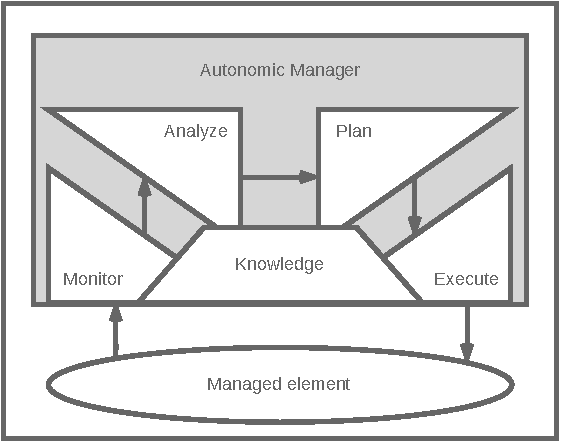
\includegraphics[width=0.6\linewidth]{images/mape-k.pdf}
    \label{fig:mapek}
\end{figure}

Cada una de estas fases son:

\begin{itemize}
    \item Monitorear (M): Esta fase se compone de la recolección, filtración y reporte de la información adquirida sobre el estado del elemento a manejar.
    \item Analizar (A): La fase de análisis se encarga de interpretar el entorno en el cual se encuentra, así como predecir posibles situaciones comunes y diagnosticar el estado del sistema.
    \item Planear (P): Durante la planificación se determinan las acciones a tomar, con el fin de llegar a un objetivo establecido a partir de una serie de reglas o estrategias.
    \item Ejecutar (E): Finalmente, se ejecuta lo planeado usando los mecanismos disponibles para el manejo del sistema. 
\end{itemize}

Es de resaltar que este modelo, aunque útil para el desarrollo de este tipo de sistemas, es bastante general en cuanto a la estructura y no usan modelos de diseño establecidos \cite{Ouareth_2018}. 

\subsubsection{Mecanismos de Descripción}

% Esta parte está más que todo para introducir el concepto de la base de conocimiento de la aplicación.
% Es decir, está orientado a dar como un ejemplo de esa base de conocimiento que tiene el "manejador" sobre la 
% plataforma

La fase de monitoreo dentro del ciclo MAPE-K es vital para el funcionamiento del manejador autonómico, pues es a partir de la información que se construirá la base de conocimiento requerida por las demás partes del ciclo. Parte de esta, está compuesta por el \textit{estado del sistema}, el cual incluye la descripción de este en un momento dado \cite{Weiss_2011}.

Existen varias implementaciones de mecanismos de auto-descripción, y la utilidad de cada uno de ellos varía dependiendo en el tipo de sistema de software que se esté usando. Para el marco del proyecto, son relevantes aquellos ,mecanismos que estén orientados a los sistemas embebidos e  IoT, algunos de estos son:

\begin{itemize}
    \item \textbf{JSON Messaging}: \citeauthor{Iancu_2022} \citeyear{Iancu_2022} plantean un protocolo que emplea mensajería entre \textit{gateways} con el fin de recibir información sobre estas. En términos simples, estas funcionan como un \textit{ping} hacia el nodo que luego retorna sus datos, al igual que los dispositivos conectados a ella, al encargado de recolectar toda esta información con el fin de construir una descripción del sistema.-
    
    \item \textbf{IoT Service Description Model}: O IoT-LMsDM, es un servicio de descripción desarrollado por \citeauthor{Wang_2021} \citeyear{Wang_2021} el cual está orientado al contexto, servicios e interfaz de un sistema IoT. De este se espera poder contar no solo con descripciones del estado del sistema en términos del ambiente, pero la funcionalidad (es decir, los \textit{endpoints} a usar) al igual que las estructuras de datos que estos consumen.
    
    \item \textbf{Adaptadores de Auto-descripción}: En este acercamiento a los mecanismos de auto-descripción, se tienen adaptadores los cuales emplean los datos generados por los sensores del componente gestionado con el fin de realizar la determinación de la arquitectura desplegada. De igual manera, este acercamiento permite realizar modificaciones a la descripción de manera manual en caso de que se detecten problemas \cite{msc_henry_2022}.

\end{itemize}

De esto podemos ver no solo las diferentes maneras en las que las implementaciones realizan las descripciones de los sistemas asociados, sino que también el alcance de estos en cuanto a lo que pueden describir.

\subsubsection{Mecanismos de Adaptación} \label{sec:MecAdap}

% Ya aquí es como definir de manera general qué es eso de los mecanismos de adaptación, qué hacen y qué características
% tienen. 
% No sé si meter ejemplos, creo que eso sería más para un estado del arte en este caso.

La adaptación, en el contexto de la computación autonómica, es la parte más importante en cuanto a la auto-gestión de un sistema de software se refiere. Así mismo, presenta el mayor reto debido a la necesidad de modificar código de bajo nivel, tener que afrontarse a incertidumbre de los efectos que pueden tener dichas alteraciones al sistema al igual que lidiar con esto en \textit{runtime} debido a los problemas que el \textit{downtime} tendría en los negocios \cite{lalanda_diaconescu_mccann_2014}. 

Esta adaptabilidad puede exponerse en múltiples puntos dentro de un sistema de software. Pueden realizarse adaptaciones a nivel de kernel, lenguaje de programación, arquitectura e incluso datos \cite{lalanda_diaconescu_mccann_2014}. 

Manteniéndose en el marco del proyecto, son relevantes aquellas soluciones relacionadas con la modificación de la arquitectura. Siendo así, se consideraron únicamente los mecanismos de adaptación de componentes, o de reconfiguración:

\begin{itemize}
    \item \textbf{Binding Modification}: Este mecanismo hace referencia a la alteración de los vínculos entre los diferentes componentes de la arquitectura. Estos tienen el objetivo de modificar la interacción entre componentes, lo que es especialmente común en implementaciones con \textit{proxies}. Este tipo de mecanismo de adaptación fue usado por \citeauthor{Kabashkin_2017} \citeyear{Kabashkin_2017} para añadir fiabilidad a la red de comunicación aérea.

    \item \textbf{Interface Modification}: Las interfases funcionan como los puntos de comunicación entre los diferentes elementos de la arquitectura. Siendo así, es posible que la modificación de estos sea de interés con el fin de alterar el comportamiento de un sistema al igual que soportar su heterogeneidad. Esto puede observarse en el trabajo desarrollado por \citeauthor{Liu_2004} \citeyear{Liu_2004} en donde se define la utilidad de dichas adaptaciones al igual que la implementación de las mismas.

    \item \textbf{Component Replacement, Addition and Subtraction}: En términos simples, este mecanismo se encarga de alterar los componentes que hacen parte de la arquitectura; de esta manera, modificando su comportamiento. Ejemplos de lo anterior pueden verse en el trabajo de \citeauthor{Huynh_2019} \citeyear{Huynh_2019}, en el cual se evalúan varios acercamientos a la reconfiguración de arquitecturas a partir del remplazo de componentes tanto a nivel individual al igual que grupal. 
    
    Este acercamiento a la mutación de la arquitectura también puede verse en el despliegue de componentes en respuesta a cambios en los objetivos de negocio de las aplicaciones, así como reacción a eventos inesperados dentro de la aplicación. Esto puede verse en trabajos como el de \citeauthor{Patouni_2006} \citeyear{Patouni_2006} donde se realizan este tipo de implementaciones. 

\end{itemize}

\subsection{Sistemas IoT Autonómicos}

Partiendo de lo anteriormente establecido, una de las áreas en las que estos conceptos de computación autonómica se ha hecho presente es el campo del IoT. Los acercamientos entre estas dos ramas de las ciencias de la computación se ha venido presentado con el objetivo de dar a los sistemas IoT la capacidad de adaptarse a su ambiente, teniendo el fin de optimizar los recursos disponibles y reducir la necesidad de interacción humana, a partir de la automatización de la configuración y procesos para mantener la disponibilidad de los servicios \cite{Ashraf2023}.

Ejemplos de estas implementaciones de propiedades autonómicas en sistemas IoT pueden apreciarse en trabajos como el de \citeauthor{Rajan2011} \citeyear{Rajan2011}, donde después de trabajar con diferentes protocolos de manejo de redes con el fin de poder realizar una administración de una red de sensores, se determinó que el manejo de un sistema de tal magnitud sería la limitante principal en el crecimiento del mismo. Esto terminó en la creación de un \textit{control loop}, el cual se encargaba de la configuración automática de la red de sensores a partir de parámetros ambientales y objetivos de calidad de servicio.

\subsubsection{Toma de Decisiones en Sistemas IoT Autonómicos}

Algo a resaltar es el tipo de métricas con las cuales se determina la validez. Estas varían dependiendo de las necesidades de las implementación al igual que los objetivos definidos por los administradores del sistema. \citeautoryear{Polanco2023}, identificaron cuatro tipos de maneras de tomar decisiones sobre un sistema IoT.

\begin{itemize}
    \item \textbf{Criterion-Driven}: Orientado principalmente al uso de algoritmos con el fin de establecer el camino a seguir en la toma de decisiones. Este acercamiento puede tener asociado un modelo matemático, algoritmos genéticos, Q-Learning, etc. dependiendo de la complejidad del sistema.
    \item \textbf{Data-Driven}: En este, a partir de datos de entrada y salida definidos, se busca determinar cómo generar datos de nuevo salida definidos dadas unas entradas. Estas están se usan principalmente en implementaciones que usan aprendizaje supervisado o sin supervisión. 
    \item \textbf{Utility-Driven}: En el caso de la utilidad, se refiere a la comparación y evaluación de diferentes alternativas de modelos matemáticos con el fin de establecer una mejor toma de decisiones. Este está relacionado con algunos conceptos usados en teoría de juegos y modelos multicriterio.
    \item \textbf{Probability-Driven}: Este hace uso de modelos probabilísticos, tales como estocásticos o bayesianos, para la toma de decisiones. Normalmente se emplean para aprendizaje no supervisado para la determinación de parámetros a partir de un punto común dados unos datos.
\end{itemize}

    
    \section{Marco Teórico}

\subsection{Internet of Things}

% Aquí es para contextualizar una de las aplicaciones de la computación embebida más que otra cosa

El Internet de las cosas, o IoT (Internet of Things); es una de las áreas de las ciencias de la computación en la cual  se embeben diferentes dispositivos en objetos del día a día. Esto les da la capacidad de enviar y recibir información con el fin de realizar monitoreo o facilitar el control de ciertas acciones \cite{Berte_2018}.

Esta tecnología, debido a su flexibilidad al igual que el alcance que puede tener, presenta una gran cantidad de aplicaciones que van desde electrónica de consumo hasta la industria. Encuestas realizadas en el 2020 reportan su uso en smart homes, smart cities, transporte, agricultura, medicina, etc. \cite{Dawood_2020}.

\subsubsection{Sistemas Embebidos}

% Tengo que contextualizar qué es lo que es la computación embebida y cual es el principio o justificación de este

Los sistemas de cómputo embebidos hacen referencia a un sistema compuesto de microcontroladores los cuales están orientados a llevar a cabo una función o un rango de funciones específicas \cite{heath2002embedded}. Este tipo de sistemas, debido a la posibilidad de combinar hardware y software en una manera compacta, se ha visto en multiples campos de la industria como lo son el sector automotor, de maquinaria industrial o electrónica de consumo \cite{deichmann_2022}.

% Extender la aplicación de la computación autonómica en los sistemas embebidos.

\subsubsection{Location-based Services}

Location-Based Services, o servicios basados en ubicación, hace referencia a aquellos servicios que integran la ubicación geográfica de un dispositivo como una parte fundamental la cual da un valor agregado al usuario \cite{Schiller2004}. Este tipo de servicios han sido principalmente usados en aplicaciones relacionas con entornos inteligentes, modelado espacial, personalización, conciencia de contexto, comunicación cartográfica, redes sociales, análisis de datos masivos, entre otros \cite{Gartner2015,alliedmarketresearch2023}. 

\subsubsection{Smart Campus}

% Y aquí es para explicar el concepto de un smart campus. Para qué se usa y de donde surge.

Un Smart Campus, equiparable con el concepto de Smart City, es una plataforma en la que se emplean tecnologías, sumado a una infraestructura física, con la cual se busca la recolección de información y monitoreo en tiempo real \cite{MinAllah2020}. Los datos recolectados tienen el objetivo de apoyar la toma de decisiones, mejora de servicios, entre otros \cite{Anagnostopoulos_2023}.

Estas plataformas, debido a su escala y alcance en cuanto a la cantidad de servicios que pueden ofrecer, requieren de 
infraestructuras tecnológicas las cuales den soporte a los objetivos del sistema. Es posible ver implementaciones orientadas a microservicios en trabajos de \citeauthor{henry_2020} \citeyear{henry_2020} donde se desarrolla una plataforma de software escalable con la cual se pueda lograr interoperatividad y alta usabilidad para todos.

% \subsection{Notación, Sintaxis y Lenguajes}

\subsection{Notación}

De manera general, notación se refiere a una serie de caracteres, símbolos, figuras o expresiones usadas con el fin de expresar un sistema, método o proceso \cite{MerriamWebsterNotation}. Más específicamente en el contexto de las ciencias de la computación, las notaciones han sido usadas para la representación de estructuras y arquitecturas en el software, como lo son lenguajes de modelado tales como UML \cite{WhatIsUML}; lenguajes de programación, como C/C++, Ruby \cite{Bansal2013}; algoritmia de manera visual \cite{RutanenKalle2018McoO}; entre otros.


\subsubsection{Gramática}

% Esto es más que nada para contextualizar la necesidad de una forma en la notación

La gramática, en el caso de los lenguajes, es un conjunto de reglas la cual es usada para describir tanto la sintaxis como la semántica de una lenguaje de programación \cite{Sebesta2012}. Siendo así, estas cumplen la función de describir una frase considerada válida dentro del contexto de un lenguaje dado \cite[p. 101]{Sipser2012-wl}. Existen varios tipos de gramática, tales como gramáticas de atributos, gramáticas libres de contexto, etc. \cite{Sebesta2012}.

\subsubsection{Sintaxis}

La sintaxis se refiere a la forma en la cual elementos, pertenecientes a un lenguaje, se estructuran de forma ordenada con el fin de formar estructuras más grandes \cite{MerriamWebsterSyntax}. En el contexto de las ciencias de la computación, esta definición se puede expresar como un conjunto de reglas con las cuales regimos la forma en que escribimos en diferentes lenguajes de programación, marcado, entre otros \cite[p. 51]{Friedman2008}.

\subsubsection{Domain-Specific Languages} % Fase 2

Los \textit{Domain-Specific Languages} (DSL), o Lenguaje de dominio específico, son lenguajes de programación empleados para un fin específico. Estos están orientados principalmente al uso de abstracciones de un mayor nivel debido al enfoque que estos tienen para la solución de un problema en específico \cite{Kelly2008}. Ejemplos de este tipo de acercamiento, en el caso del modelado (\textit{Domain-specific modeling}), pueden observarse en los diagramas de entidad relación usados en el desarrollo de modelos de base de datos \cite{Celikovic2014ADF}. 

\subsection{Serialización de Datos}

La serialización de datos se refiere a la traducción de una estructura de datos a una manera en la que pueda ser almacenada o transmitida de manera eficiente \cite{mozillaSerialization}. Este proceso ha sido, principalmente, adoptado por lenguajes de programación orientada a objetos, en donde existe un soporte nativo, tales como Go, JavaScript, o PHP; o existe algún tipo de framework o librería que permite hacerlo, como lo es en el caso de C/C++, Rust o Perl.

\subsubsection{Métodos de Serialización de Datos}

Dentro del ámbito de la programación, se encuentran diversas opciones en cuanto a formatos y técnicas empleadas para la serialización de datos. Cada uno de estos enfoques presenta sus particularidades, lo que resulta en ventajas y desventajas específicas, las cuales deben ser consideradas según las necesidades del proyecto. Las dos opciones principales, en cuanto a la serialización de datos, son:

\begin{itemize}
    \item \textbf{Serialización en Formato de Texto}: Esta forma de serialización emplea un formato legible por humanos, generalmente utilizando caracteres y símbolos. Este enfoque es especialmente útil cuando se necesita que los datos sean legibles, y editables, directamente por humanos, lo que los hace adecuados para la configuración de aplicaciones y la comunicación entre sistemas heterogéneos; o cuando se requiere tener compatibilidad entre diferentes sistemas y lenguajes de programación \cite{Grochowski2019}.
    \item \textbf{Serialización Binaria}: Esta implica la representación de datos en un formato binario. Este enfoque es altamente eficiente en cuanto a espacio y velocidad, pero no es legible por humanos. Los formatos de serialización binaria, están diseñados para minimizar el tamaño de los datos serializados y optimizar el rendimiento en aplicaciones donde la velocidad y la eficiencia son críticas, sacrificando la estandarización e interoperatividad con otras implementaciones de este tipo de serialización \cite{Grochowski2019}.
\end{itemize}
    
    \section{Metodología de la Investigación}

Para el desarrollo del trabajo de grado, se propuso un modelo de prototipado iterativo compuesto de 5 fases (Ver fig. \ref{fig:met}), que permitió avanzar a medida que se fue completando la fase anterior y permitió el poder iterar sobre lo que se ha desarrollado anteriormente.

\begin{figure}[H]
    \centering
    \caption{\\Metodología de investigación}
    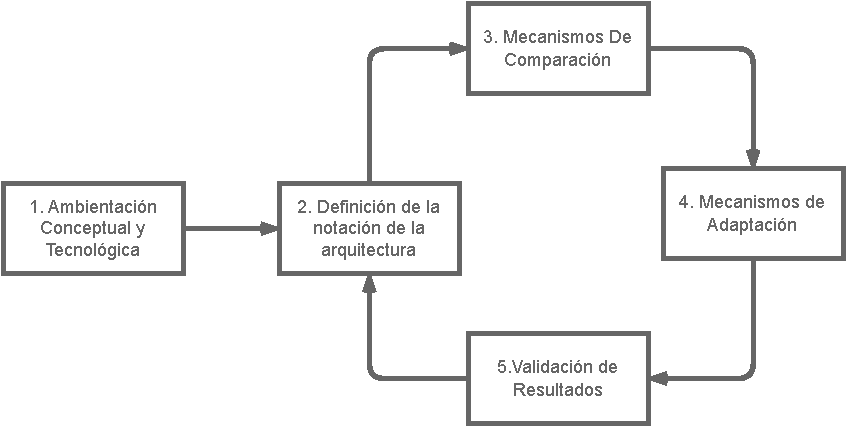
\includegraphics[width=0.7\linewidth]{images/Metodologia.pdf}
    \label{fig:met}
\end{figure}

\subsection{Ambientación Conceptual y Tecnológica}

La primera fase de la metodología se basó en la revisión de la literatura, al igual que de lo presente en la industria, lo anterior fué necesario para cubrir las bases tanto conceptuales como técnicas requeridas para el desarrollo del proyecto. 

\subsubsection*{Actividades}

\begin{enumerate}
    \itemsep-2mm
    \item Identificación de las características principales de un sistema auto-adaptable.
    \item Análisis de los mecanismos de adaptación de la arquitectura.
    \item Análisis los algoritmos empleados para la comparación de las arquitecturas.
    \item Determinación de los criterios de selección para el lenguaje de notación.
    \item Evaluación de los posibles lenguajes de programación para la implementación a realizar.
\end{enumerate} 

\subsubsection*{Productos}

\begin{enumerate}
    \itemsep-2mm
    \item Lista de criterios de selección para el lenguaje de notación.
    \item Evaluación de los posibles lenguajes de programación para la implementación.
\end{enumerate}

\subsection{Definición de la notación de la arquitectura}

La segunda fase consistió en la definición del cómo se realiza la declaración de la arquitectura. Partiendo de los criterios de selección establecidos en la fase 1, se determinó un lenguaje de notación el cual permitió definir la arquitectura objetivo a alcanzar, al igual que la gramática correspondiente para poder realizar dicha declaración. 

\subsubsection*{Actividades}

\begin{enumerate}
    \itemsep-2mm
    \item Selección del lenguaje de marcado a usar a partir de los criterios establecidos.
    \item Definición de la gramática a usar para la definición de la arquitectura.
    \item Determinación de como se realizará la representación de los componentes y partes de la arquitectura.
    \item Implementación de una validador de la notación propuesta.
\end{enumerate}    

\subsubsection*{Productos}

\begin{enumerate}
    \itemsep-2mm
    \item Notación a usar para la declaración de los requerimientos de las aplicaciones.
    \item Validador de los archivos de configuración de la notación definida
\end{enumerate}

\subsection{Mecanismos De Comparación}

Durante la tercera fase del proyecto, se buscó determinar e implementar cómo se realiza la comparación entre el estado de la arquitectura obtenido durante la auto-descripción de la misma y el objetivo establecido. Así mismo, y con el fin de reportar a los administradores de los sistemas, también fue necesario definir los \textit{niveles} de similitud entre las 2 arquitecturas.

\subsubsection*{Actividades}

\begin{enumerate}
    \itemsep-2mm
    \item Selección del mecanismo de comparación a usar para evaluación de estado de la arquitectura.
    \item Implementación del mecanismo de comparación seleccionado.
    \item Determinación de los diferentes niveles de similitud entre arquitecturas.
\end{enumerate}    

\subsubsection*{Productos}

\begin{enumerate}
    \itemsep-2mm
    \item Implementación de un mecanismos que permita establecer el estado del sistema.
    \item Implementación de una comparación entre el estado de referencia y el estado actual.
\end{enumerate}

\subsection{Mecanismos De Adaptación}

La cuarta fase del proyecto fue orientada a la selección, al igual que la implementación en Smart Campus UIS, del conjunto de mecanismos de adaptación de la arquitectura. 

\subsubsection*{Actividades}

\begin{enumerate}
    \itemsep-2mm
    \item Definición el conjunto de mecanismos de adaptación.
    \item Implementación el conjunto de mecanismos de adaptación seleccionados.
\end{enumerate}  

\subsubsection*{Productos}

\begin{enumerate}
    \itemsep-2mm
    \item Implementación de un servicio encargado de la planeación para la ejecución de los mecanismos de adaptación definidos
    \item Implementación de un servicio encargado de la ejecución de las acciones planeadas.
\end{enumerate}

\subsection{Validación De Resultados}

La fase final del proyecto se centró principalmente en la realización de pruebas de los mecanismos implementados, los resultados obtenidos al igual que la documentación de todo lo que se desarrolló durante el proyecto.

\subsubsection*{Actividades}

\begin{enumerate}
    \itemsep-2mm
    \item Realización de las pruebas del funcionamiento de la implementación realizada con diversas arquitecturas objetivo.
    \item Recopilación la documentación generada durante el desarrollo de cada una de las fases del proyecto.
    \item Compilación de la documentación para generar el documento final.
    \item Correcciones y adiciones para la presentación final del proyecto de grado.
\end{enumerate}  

\subsubsection*{Productos}

\begin{enumerate}
    \itemsep-2mm
    \item Validación del funcionamiento de los mecanismos implementados.
    \item Código fuente de los diferentes servicios y librerías implementadas durante el transcurso del proyecto
    \item Documento final detallando el desarrollo del proyecto
    \item Presentación para la sustentación del proyecto
\end{enumerate}
    
    
    \section{Lenguajes de Descripción de Arquitectura}

\subsection{La necesidad de una arquitectura de referencia}

La necesidad de una arquitectura de referencia, o arquitectura objetivo; es una parte esencial dentro de la computación autonómica. Esta forma parte de la base de conocimiento (K), y, de manera indirecta, de los objetivos del administrador del sistema \cite[p. 24]{lalanda_diaconescu_mccann_2014}. 

Con el fin de establecer un objetivo para el sistema autonómico, fue necesario determinar una manera de realizar la declaración de dicha arquitectura, que estableciera un estado de referencia. De esta manera, podría evaluarse el estado del sistema en tiempo de ejecución,  y así tomar las acciones necesarias para adaptarlo hacia el estado de referencia. 

Ahora, fue también necesario establecer el punto desde el cual se lleva a cabo la comparación entre los estados del sistema. Esto guió la búsqueda para determinar el como se realizó la declaración de los estados objetivo de Smart Campus UIS, al igual que los datos a recolectar.

Siendo así, y dados los objetivos que buscan cumplir los ecosistemas inteligentes para la toma de decisiones \cite{Anagnostopoulos_2023}, se enfocó no sobre la arquitectura sobre la cual trabaja la plataforma, sino sobre las aplicaciones desarrollándose sobre esta. Es decir, los datos requeridos. Son las necesidades definidas por las aplicaciones, las descritas y usadas para evaluar el estado del sistema. Siendo así, que el enfoque debía estar orientado a cumplir con las necesidades de los datos establecidas por Smart Campus. Esto se expondrá de manera más clara durante las fases de comparación y adaptación.

\subsection{Criterios de selección}

Con el fin de establecer la notación a usar para la declaración de las arquitecturas objetivo, se establecieron unos lineamientos con los cuales se realizaría la evaluación de las diferentes notaciones ya desarrolladas anteriormente. De esta manera se podría escoger la manera a representar los modelos, o en el caso de ser necesario, establecer los criterios por el cual se podría desarrollar uno.

% En la tabla \ref{tab:criterios}, se presentan los criterios usados para la selección, con su respectiva explicación y valor considerado para la selección.

\begin{table}[H]
    % \small
    \centering
    \vspace{-4mm}
    \caption{\\Criterios usados para la determinación de la notación a utilizar} \label{tab:criterios}
    % \vspace{4mm}
    \begin{tabular}{lm{4.7cm}m{0.60\linewidth}c}
        \hline
        \multicolumn{1}{l}{} &
        \multicolumn{1}{c}{\textbf{Criterio}} &
        \multicolumn{1}{c}{\textbf{Explicación}} \\ \hline
        C1 & \centering Describir la arquitectura de un sistema IoT &
        Este criterio es una base a establecer con el fin de descartar aquellos lenguajes de notación generales o no necesariamente usados para la descripción de arquitecturas IoT.  \\ 
        C2 & \centering  Permitir la especificación de la ubicación del componente &
        La especificación de la ubicación de los componentes es importante en los sistemas IoT, especialmente dentro del contexto del proyecto en el cual se está trabajando con un Smart Campus; ya que los componentes pueden estar distribuidos en diferentes ubicaciones físicas y la evaluación de su integridad puede depender de su presencia en un lugar dado. \\ 
        C3 & \centering Habilitar el modelado del componente a nivel de sus entradas &
        Es importante poder describir las entradas de los componentes, específicamente los datos que manejan, así como su rol dentro del sistema.  \\ 
        C4 & \centering Modelar el comportamiento de los componentes &
        La notación debe permitir modelar el comportamiento de los componentes, de manera que se puedan entender sus interacciones y su función en el sistema IoT. Dentro del contexto del proyecto, no es tan relevante, ya que no se está evaluando la funcionalidad del sistema, sin embargo, para futuros trabajos, podría facilitar la extensión de Smart Campus UIS.  \\ 
        C5 & \centering Posibilitar el establecer los estados de los componentes &
        La notación debe poder definir los estados de los componentes. Estos estados pueden ser tanto de comportamiento o operacionales.  \\ 
        C6 & \centering Permitir de exportar el modelo descrito a gráficas u otros formatos &
        Es importante que la herramienta permita exportar el modelo descrito en diferentes formatos para facilitar su integración con otras herramientas y sistemas, y para permitir su visualización en diferentes formatos. \\ \hline
    \end{tabular}
    \vspace{-4mm}
\end{table} 


\subsection{Búsqueda de Alternativas}

Una vez establecidos los criterios de selección, se realizó una exhaustiva búsqueda de alternativas disponibles en la literatura y en la industria para describir arquitecturas de sistemas IoT. Este proceso se realizó a partir de la revisión en diferentes bases de datos, como \textit{Scopus}; al igual que algunas de las revistas especializadas en el tema, y el internet en general.

Durante la búsqueda, se identificaron una gran variedad de opciones. Sin embargo, la gran mayoría de estas se filtraron, o descartaron; a partir de los criterios de selección establecidos. Esto se debió a que los LDAs usados tanto en la industria y academia, como AADL (Architecture Analysis and Design Language), tienen un enfoque a los campos de aviónica, equipos médicos y aeronáutica (lo que complicaría su implementación hacia sistemas de software IoT) \cite{aadl_web, aadl_pdf}; o SysML, que son bastante genéricos y abarcan hardware, software e incluso personas y procesos \cite{omgsysml_2015}.

Es así como, de las posibles opciones de notación, se seleccionaron cinco, las cuales fueron evaluadas con el fin de determinar si alguna de estas hubiera podido ser usada, o si era necesario desarrollar una notación propia para el proyecto. A continuación, se presentan las alternativas evaluadas:

\begin{itemize}
    \item \textbf{MontiThings:} Basado en MontiArc, otro LDA más general; está diseñado para el modelado y prototipado de aplicaciones de IoT. Este realiza las descripciones de sus arquitecturas en un modelo componente-conector, donde los componentes están compuestos por otros componentes; y los conectores definen la manera en la que se comunican dichos componentes a nivel de los datos y la dirección de los mismos. \cite{MontiThings, MontiThingsRepo}
    \item \textbf{Eclipse Mita}: Mita, creado por la Eclipse Foundation; es un lenguaje de programación orientado al facilitar la programación de sistemas IoT. Aunque como tal no es un LDA, está orientada a la descripción de los componentes y el comportamiento del sistema establecido, de esta manera, puede generar el código que debe correr en los dispositivos embebidos \cite{Mita}. 
    \item \textbf{SysML4IoT:} Es un perfil de SysML\footnote{Los perfiles se refieren a extensiones a UML, en este caso es una extensión de SysML en sí \cite{Charles2007}.} en el cual se usan estereotipos de UML con el fin de abstraer las diferentes partes de los sistemas de IoT. Al igual que SysML, este permite el modelado más allá de dispositivos incluso llegando a personas y procesos, con la diferencia del enfoque dado al \textit{dominio de IoT} \footnote{El \textit{dominio del IoT}, hace referencia al \textit{Architecture Reference Model} establecido por IoT-A, un consorcio Europeo el cual buscaba el establecer un modelo para la interoperatividad de dispositivos IoT. \cite{IoTA2014}} \cite{SysML4IoT2016}.
    \item \textbf{ThingML:} Similar a Mita, ThingML, es un lenguaje de modelado el cual tiene capacidades de generar el código requerido por los dispositivos embebidos. En términos del proyecto, este permite el modelado de los sistemas de IoT a partir de \textit{state machine models}\footnote{Los \textit{state machine model}, también conocidas como Autómatas Finitos; son modelos matemáticos que describen todos los posibles estados de un sistema a partir de unas entradas dadas \cite{StateMachine2023}. } los cuales permiten describir los componentes del sistema al igual que el comportamiento de estos \cite{ThingML2016}.
    \item \textbf{IoT-DDL}: Iot-DDL es un LDA, implementado en XML, que describe objetos dentro de los ecosistemas IoT con base en sus componentes, identidad y servicios entre otros. Este tiene la capacidad de describir parte de la base de conocimiento que tienen los diferentes componentes (Principalmente relaciones y asociaciones entre componentes) \cite{Ahmed2018}.
\end{itemize}

Una vez seleccionadas las alternativas a evaluar, se utilizó la matriz de evaluación en la tabla \ref{tab:evaluation} para determinar la solución ideal para el desarrollo del proyecto. 

\skipline
\skipline
\skipline
\skipline

\begin{table}[H]
    \centering
    % \vspace{-4mm}
    \caption{\\Evaluación de las alternativas en función de los criterios establecidos} \label{tab:evaluation}
    % \vspace{4mm}
    \begin{tabular}{cccccc}
    \hline
    \multicolumn{1}{l}{} &
      \multicolumn{1}{l}{MontiThings} &
      \multicolumn{1}{l}{Eclipse Mita} &
      \multicolumn{1}{l}{SysML4IoT} &
      \multicolumn{1}{l}{ThingML} &
      \multicolumn{1}{l}{IoT-DDL} \\ \hline
      C1 & ✓ & ✓ & ✓ & ✓ & ✓ \\
      C2 & ✗ & ✗ & ✗ & ✗ & ✗ \\
      C3 & ✓ & ✓ & ✓ & ✓ & ✓ \\
      C4 & ✓ & ✓ & ✓ & ✓ & ✗ \\
      C5 & ✓ & ✓ & ✗ & ✓ & ✗ \\
      C6 & ✗ & ✗ & ✗ & ✓ & ✗ \\ \hline
    \end{tabular}
    % \vspace{-4mm}
\end{table}

Partiendo de los resultados de la evaluación, se puede apreciar que ninguno de estos LDA cumple con los criterios establecidos para el proyecto. Aunque estos están orientados hacia la descripción y desarrollo de sistemas IoT, no están enfocados hacia su contexto en términos de aplicación más allá de la definición de comportamiento. Esto se debe a los objetivos de cada una de estas notaciones, de una u otra manera; buscan el representar como tal el sistema IoT en términos de su funcionalidad técnica y no la aplicación en si. 

\subsection{Un nuevo modelo para Smart Campus}

Dado que no hay una alternativa que se adapte completamente a las necesidades del proyecto, se tuvo que definir una notación propia, la cual permita modelar las arquitecturas a nivel de aplicación bajo el contexto de un Smart Campus, tomando en cuenta los criterios definidos como guía para el desarrollo.

Primeramente, fue necesario definir un metamodelo que permitiera establecer la manera en la que se ven estas arquitecturas. Para ello, y partiendo de la implementación a realizar, se apoyó parcialmente en el modelo establecido por \citeA[p. 63]{msc_henry_2022}. 

\begin{figure}[H]
    \centering
    \caption{\\Versión 2 del modelo concepto planteado por \protect\citeauthor{msc_henry_2022}}
    \label{fig:henrymodelo}
    \vspace{2mm}

    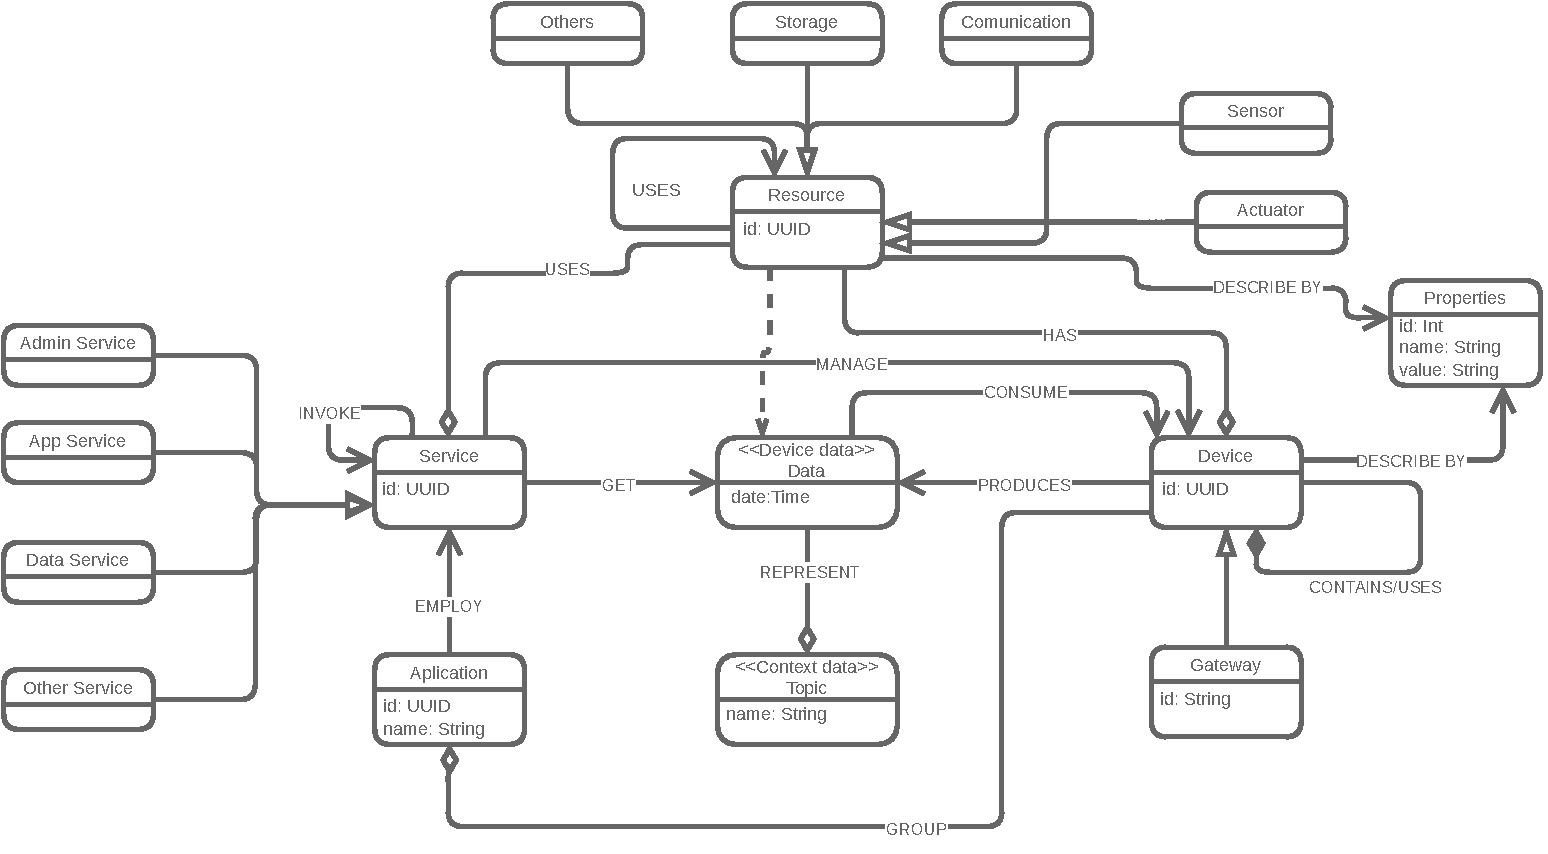
\includegraphics[width=\linewidth]{images/HenryModelo.pdf}
\end{figure}

Basarse en el modelo de la figura \ref{fig:henrymodelo}, da la capacidad de describir a un nivel técnico un sistema IoT. Ahora, aunque se podría usar para el desarrollo del proyecto, fue necesario modificarlo, con el fin de acercarnos más hacia la descripción de un sistema IoT a nivel de aplicación. 

El primer paso fue establecer el contexto de los dispositivos. Esto específicamente se refiere al criterio \textit{C2} de la tabla \ref{tab:criterios}, en donde, dada la necesidad de establecer la ubicación geográfica en algunas de las aplicaciones de los Smart Campus, era necesario poder describir los lugares pertenecientes a la aplicación.

Así mismo, se cubre el criterio \textit{C3} cambiando las propiedades del dispositivos de una clase, externa a los dispositivos; a un atributo, interno, el cual le permite a los componentes manejar su propia información en cuanto a los datos que estos manejan. Estas propiedades pueden referirse a las entradas que tienen, en el caso de ser actuadores o procesadores de la información; o a los valores que reportan al sistema en el caso de ser sensores.

Ahora, algo importante a tener en cuenta, es la manera en la que se están reportando los datos desde los sensores hacia Smart Campus UIS. Esto se debe a la necesidad de tener en cuenta los datos a los cuales tenemos realmente acceso desde cada uno de los dispositivos.

Cada uno de los dispositivos de Smart Campus, reporta un `JSON` similar al presente en la figura \ref{fig:jsonSCU}. Este mensaje contiene información que permite identificar al dispositivo, gracias al \textit{UUID}; al igual que el momento y los datos que este reporta.

\begin{figure}[H]
    \centering
    \caption{\\Mensaje JSON enviado por los dispositivos en Smart Campus UIS }
    \cite{SmartCampusGithub}
    \label{fig:jsonSCU}
    \begin{tabular}{c}
        \setstretch{1}
        \small
        \begin{lstlisting}[language=Json]
            {   
            "deviceUUID": "1",
            "topic": "temperatura",
            "timeStamp": "06-01-2024 10:39:02",
            "values": {
                "temperature": 10.0,
                "co2": 15.0,
                "location": "AP2" 
            },
            "status": "OK",
            "alert": false  
            }
        \end{lstlisting}
    \end{tabular}
\end{figure}

Es importante destacar que, aunque contamos con suficiente información para identificar los dispositivos, en estos mensajes no está presenta información crucial para el mapeo físico de los dispositivos. Por lo tanto, será necesario proporcionar manualmente estos datos durante la etapa de adaptación para llevar a cabo los ajustes necesarios en la arquitectura.

Partiendo de esto, se desarrolló el UML presente en la figura \ref{fig:metamodelo}. La base de este es la aplicación (\textit{\texttt{Application}}). Este contiene, a partir de una ubicación raíz, todas las demás locaciones (\textit{\texttt{location}}) pertinentes para el correcto funcionamiento de esta.

\begin{figure}[ht]
    \centering1
    \caption{\\Versión 1 del metamodelo planteado para SCampusADL}
    \label{fig:metamodelo}
    \vspace{2mm}
    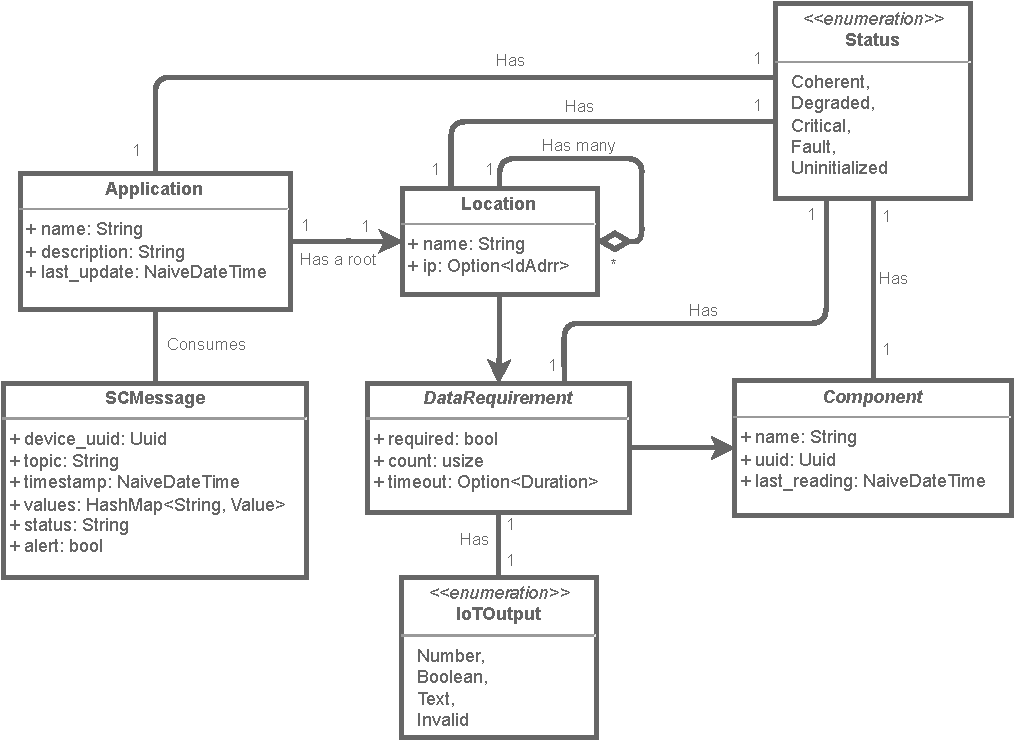
\includegraphics[width=\linewidth]{images/Metamodel B.pdf}
\end{figure}

Las locaciones, tienen una serie de requerimientos de datos (\texttt{\textit{DataRequirements}}), las cuales son las representaciones lógicas, o de software, de las necesidades de la aplicación. Estos pueden ser de 2 tipos: requeridos, que son aquellos con los cuales de no tenerlos, la aplicación no podría funcionar correctamente; y los opcionales, los cuales, aunque buenos de tener, no impiden el funcionamiento.

Cada uno de estos requerimientos de datos, contiene la cantidad de dispositivos, y a su vez datos, requeridos por la locación, al igual que el tipo de datos esperado (\textit{\texttt{IoTOutput}}), y el que el tiempo máximo permitido entre reportes de datos. 

Los requerimientos de datos, llevan un registro de los componentes (\textit{\texttt{Component}}) que han reportado datos en la locación. Esto permite evaluar cada uno de estos, y en la misma medida, determinar el estado (\textit{\texttt{Status}}) de cada una de las locaciones registradas en la aplicación. Estos estados buscan describir qué tan diferente es lo observado de lo esperado al igual que la validez de cada una de las partes. 

Ahora, las aplicaciones, en cierta medida, con el fin de llevar el registro de los datos enviados, consumen el mensaje JSON visto en la figura \ref{fig:jsonSCU}. Este ha sido deserializado y mapeado en \textit{\texttt{SCMessage}}. De esta manera, se podrá trabajar de manera sencilla en el procesamiento y actualización del estado de las aplicaciones.

De este modelo, se desarrolló e implementó una librería, apodada \textit{StarDuck}\footnote{El código fuente de la librería puede encontrarse en \url{https://github.com/ChipDepot/StarDuck}, y su respectivo paquete en crates.io, en \url{https://crates.io/crates/starduck}.}. Esta librería contiene todas las estructuras de datos definidas en el modelo, las cuales serán usadas por el resto de los servicios y aplicativos necesarios para la declaración, evaluación y adaptación de las arquitecturas de software en el proyecto. 


\subsection{Sintaxis de la notación}

Partiendo de esto, lo siguiente que se realizó fue la definición de la sintaxis de la notación a usar, basados en lo definido por el metamodelo. Para esto, se decidió usar \texttt{YAML}, un lenguaje de serialización de datos orientado a la legibilidad, reconocido y usado principalmente para la creación de archivos de configuración \cite{YAML2023}. 

La sintaxis, como puede observarse en la figura \ref{fig:rail-base}, se compone de 2 partes: \texttt{Application}, donde se declara la aplicación; y \texttt{Locations}, en donde se define el contexto geográfico al igual que las necesidades de datos de estas.

\begin{figure}[H]
    \centering
    \caption{\\Diagrama de rail de la sintaxis definida para la notación de SmartCampusADL}
    \label{fig:rail-base}
    \vspace{2mm}
    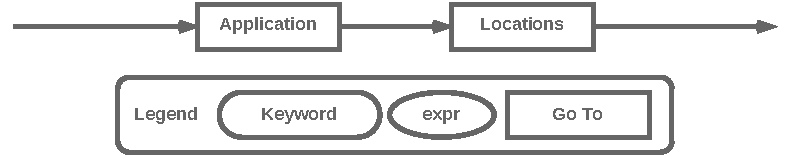
\includegraphics[width=\linewidth]{images/Railroad Base.pdf}
\end{figure}

Esta primera parte, como puede observarse en la figura \ref{fig:rail-app} se refiere al nombre que se usará para referirse a la aplicación al rededor de todos los servicios, y una descripción opcional con fines de documentación.

\begin{figure}[H]
    \centering
    \caption{\\Diagrama de rail de la sintaxis de declaración de la aplicación}
    \label{fig:rail-app}
    \vspace{2mm}
    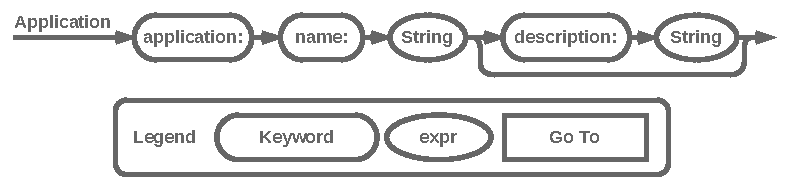
\includegraphics[width=\linewidth]{images/Railroad Application.pdf}
\end{figure}

Para especificar las \texttt{locaciones} dentro del contexto de la aplicación, se definió la sintaxis que puede observarse en la figura \ref{fig:rail-location}. Partiendo de la locación raíz de la aplicación, podrán declararse \textit{n} cantidad de locaciones, cada una con un nombre diferente.

\begin{figure}[H]
    \centering
    \caption{\\Diagrama de rail de la sintaxis definida para la notación del contexto geográfico de la aplicación}
    \label{fig:rail-location}
    \vspace{-2mm}
    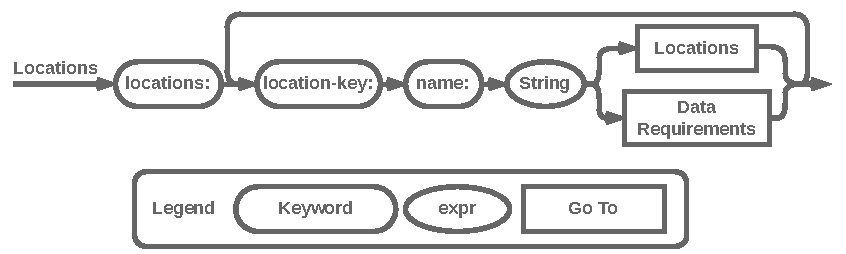
\includegraphics[width=\linewidth]{images/Railroad Locations Alt.pdf}
\end{figure}

Las locaciones pueden funcionar de una de dos maneras. La primera es como agrupadores de otras locaciones, que puede verse como varios edificios de un campus o como varios pisos de un edificio, dependiendo de la granularidad que requiera la aplicación. Y, la segunda son puntos de origen de datos requeridos por la aplicación, reportados por diversas clases de dispositivos presentes.

Los requerimientos de datos, como se puede ver en la figura \ref{fig:rail-data-req}, están compuestos de varias partes. Las \texttt{data-key} se refieren al nombre del requerimiento de dato de la locación. Se espera que estos sean los mismos usados en la parte de \texttt{values} vista en los mensajes de la plataforma Smart Campus de la figura \ref{fig:jsonSCU}.

\begin{figure}[H]
    \centering
    \caption{\\Diagrama de rail de la sintaxis definida para la notación de los componentes de la aplicación}
    \label{fig:rail-data-req}
    \vspace{-2mm}
    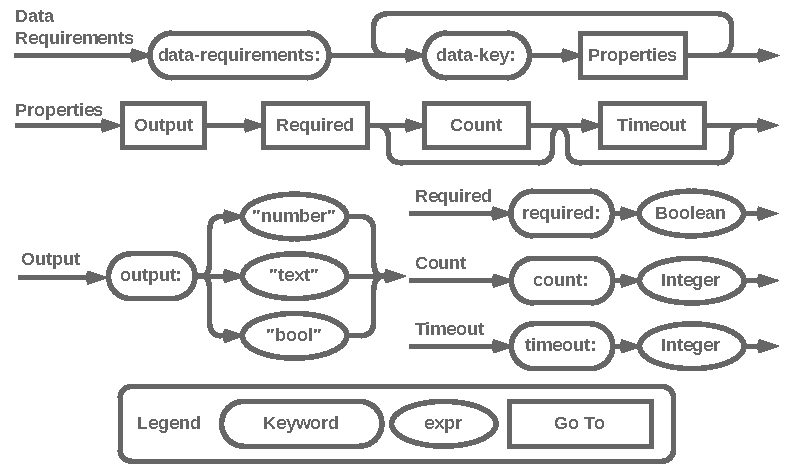
\includegraphics[width=0.9\linewidth]{images/Railroad Data Requirements.pdf}
\end{figure}

A continuación, se procedería a definir las propiedades de dicho requerimiento de datos. Para esta primera versión de la notación, se han establecido las 4 cuatro propiedades vistas en el modelo (ver figura \ref{fig:metamodelo}), dos son obligatorias para la declaración. La primera es \texttt{output}, que hace referencia al tipo de dato esperado \footnote{Este output, en el modelo es el \textit{enum} \texttt{IoTOutput}, que representa los tipos de datos.}, y la segunda es \texttt{required}, que especifica si el requerimiento es obligatorio u opcional. Las otras dos propiedades opcionales: \texttt{count}, que representa la cantidad de fuentes de datos necesarias en la ubicación, y \texttt{timeout}, que indica el tiempo máximo entre los informes de datos. En ambos casos, de no declararlas, se tomaría como valor por defecto 0.

El resultante de esta notación serían archivos de declaración de arquitecturas, en formato YAML, similares a la que se puede observar en la figura \ref{fig:YAML-ADL}.

\begin{figure}[ht]
    \centering
    \caption{\\YAML de una posible aplicación de monitorio}
    \label{fig:YAML-ADL}
    \begin{tabular}{c}
        \setstretch{1}
        \small
        \lstinputlisting[language=YAML]{metamodel/modelV2.yaml}
    \end{tabular}
\end{figure}

Con esto hemos creado un marco sólido para representar las aplicaciones de Smart Campus UIS. Este enfoque bien definido, permitirá avanzar en el desarrollo de las funcionalidades para comparación de los modelos, y la implementación de los mecanismos de adaptación a usar. 

\input{sections/2. LDA/6. validación.tex}




    
    \section{Estado Actual Frente al de Referencia}

\subsection{Conociendo el estado actual}

Con la notación de las arquitecturas objetivo establecidas, al igual que el desarrollo del módulo encargado de la construcción y validación de los archivos de configuración; lo siguiente era la definición del proceso de la comparación entre la arquitectura actual y la arquitectura de referencia. Este proceso, permitirá evaluar el estado del sistema y, por consiguiente, establecer las acciones a tomar con el fin de adaptar la arquitectura hacia el estado objetivo establecido.

Esto requiere conocer el estado actual del sistema, al igual que el conocer el estado objetivo. Siendo así, y ya teniendo la posibilidad de declarar las necesidades de la aplicación, lo siguiente es establecer una manera de determinar el estado del sistema. Dado el enfoque hacia los datos recolectados, es necesario el precisar la manera en la que conoceríamos en qué estado se encuentra el sistema.

Lo primero era el identificar los puntos de acceso por los cuales podríamos acceder a los datos. En el caso de Smart Campus UIS, y teniendo en cuenta que el modelo que se definió depende de los mensajes enviados por los dispositivos, como se observa en la figura \ref{fig:ArquitecturaSmartCampus}, existen dos opciones para procesar estos mensajes. 

La primera, es consultar los mensajes enviados usando uno de los endpoints del servicio \texttt{data\_microservice}, lo que da acceso a todos los mensajes registrados. Y, la segunda, usando el mismo bus de datos, empleado por los servicios de la plataforma, lo que permitiría el acceso, incluso de manera más directa, a los mensajes a medida que estos son enviados.

\begin{figure}[ht]
    \centering
    \caption{\\Arquitectura del prototipo de Smart Campus definido por }\citeA{msc_henry_2022}
    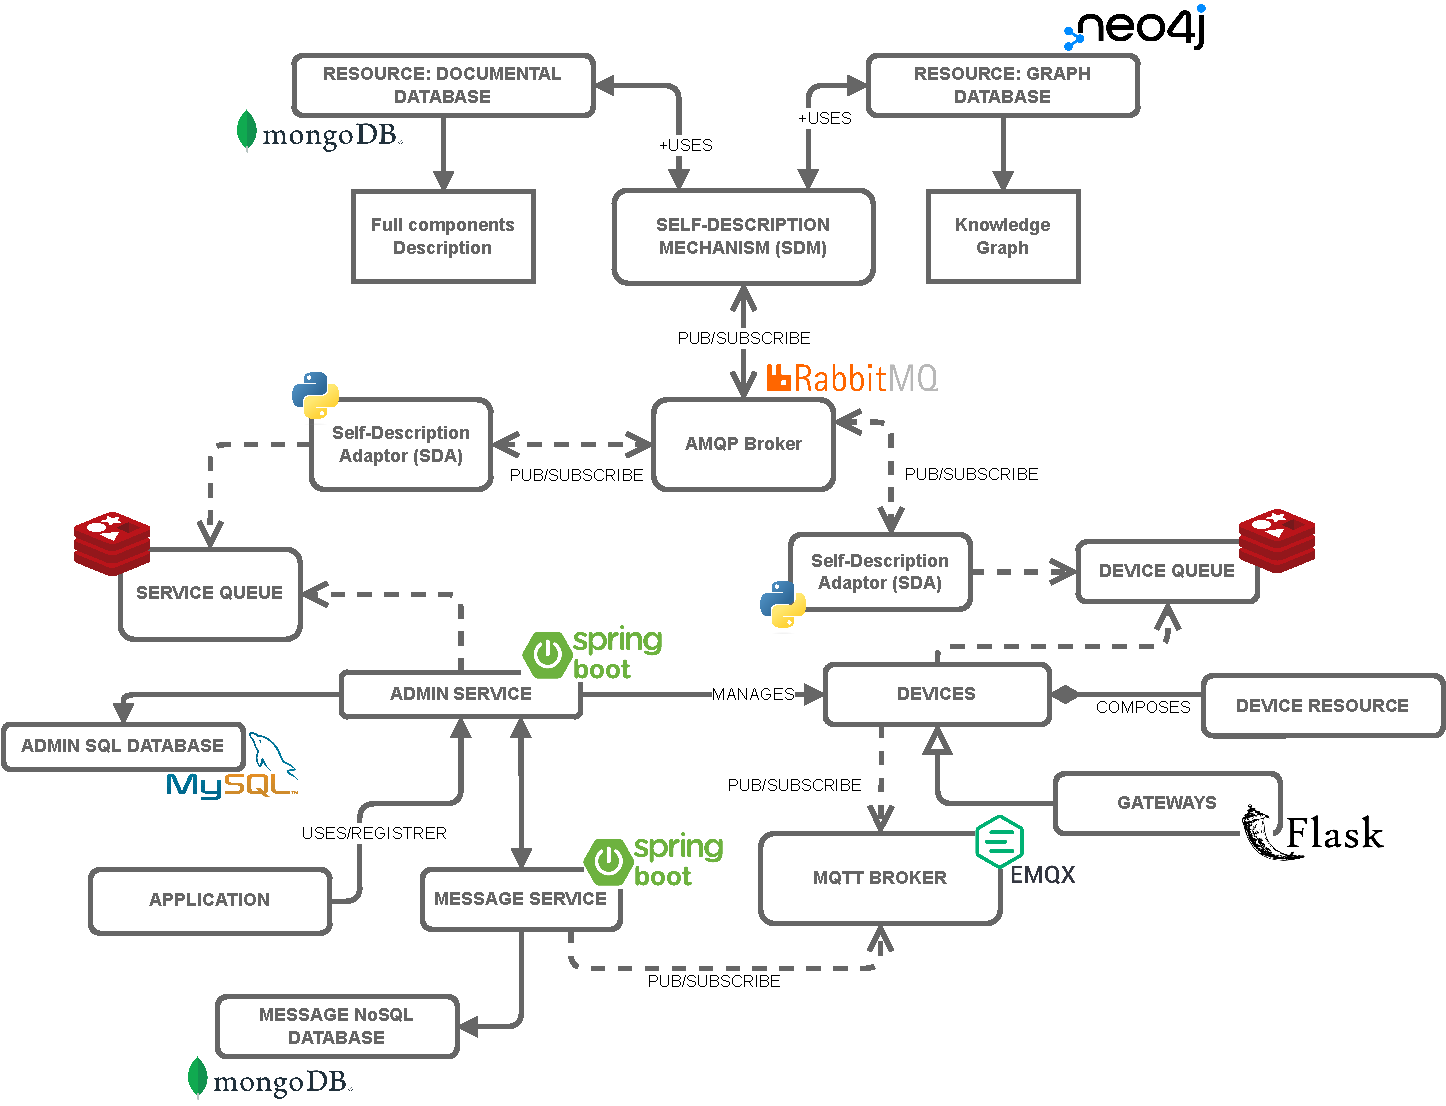
\includegraphics[width=\linewidth]{images/ArquitecturaSmartCampusUis.pdf}
    \label{fig:ArquitecturaSmartCampus}
\end{figure}

Ahora, cada una de las maneras de acceder a los datos es viable, y podría permitir la implementación correspondiente para determinar el estado del sistema. Sin embargo, de entre las dos opciones, se escogió el procesamiento de los mensajes enviados por los dispositivos, enviados por MQTT. 

Esto se debe a varios factores, principalmente, debido a cómo se consultan los mensajes desde el endpoint. Para realizar esta consulta, es necesario conocer el \textit{UUID} del dispositivo a consultar lo que, como se evidenció durante la validación de los requerimientos de datos en la sección \ref{sec:validation}, no es posible.

Aunque sería posible el realizar una modificación al servicio para poder ver todos los mensajes de los dispositivos, esto también podría presentar problemas por la manera en la que estos se listan. Ya que los mensajes se muestran todos en simultaneo, y no poseen una manera diferenciar 2 mensajes, más allá de su contenido (que no es necesariamente único); tendríamos que guardar todos los mensajes ya procesados y descartarlos cada vez que se consulte el endpoint, lo que generaría un \textit{overhead} el uso de los recursos tanto de memoria como de procesamiento.

Siendo así, queda como opción el broker MQTT para la consulta de los mensajes. Este acercamiento permite el procesamiento, en tiempo real, de los mensajes enviados por los dispositivos, sin la necesidad de conocerlos; al igual que un aprovechamiento de los recursos ya que, una vez procesados, podemos librar el espacio usado. Esto le da una característica al proyecto en forma de una especie de \textit{plug-in}, puesto que, al no requerir modificaciones sobre la plataforma, esta puede funcionar sin ninguna afectación en su estado actual.

Partiendo de lo anterior, se realizó el diseño e implementación de un servicio encargado de procesar los mensajes que están siendo enviados por, y a, cada uno de los dispositivos registrados en Smart Campus UIS. 




\subsection{Centralizando los Datos} \label{sec:Centering}

Lo primero para la implementación del observador, era determinar como este tendría acceso al estado de referencia. Hasta el momento, únicamente \textit{Lexical} tiene el contexto definido por el usuario, por lo que era necesario definir una manera mediante la cual otros servicios puedan acceder a este.

Partiendo de la división de responsabilidades, se estableció el implementar un agregador, que contenga el estado definido por el usuario; desde el cual otros servicios puedan acceder a estos datos. 

Esto tiene dos ramificaciones adicionales. La primera, es que abre a la posibilidad de declarar más de una aplicación en simultaneo, usando el agregador como un \textit{hub} que permita guardar y consultar los estados de las aplicaciones que se registren, teniendo una instancia de observador por cada una de ellas.

La segunda, posibilita el usar este agregador para almacenar los estados actuales reportados por el observador. Esto se debe a que, las condiciones para evaluar el estado de las aplicaciones, se encuentran en las propiedades definidas por el usuario durante la declaración del estado de referencia. Siendo así, es posible ver el estado objetivo a partir de las propiedades; y el estado actual basado en la evaluación de los componentes registrados en los requerimientos de datos.

De lo anterior, podemos planear un diagrama, visto en la figura \ref{fig:StarDuckMini}, que refleje el estado actual de la arquitectura del proyecto.

\begin{figure}[ht]
    \centering
    \caption{\\Arquitectura actual del proyecto con el agregador}
    \label{fig:StarDuckMini}
    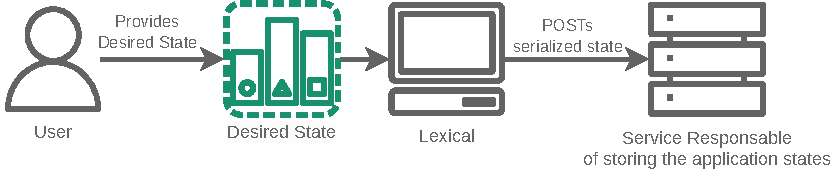
\includegraphics[width=0.9\linewidth]{images/StarDuckMini.pdf}
\end{figure}

La implementación de este agregador, apodado \textit{Bran}\footnote{El código fuente de Bran puede encontrarse en el repositorio \url{https://github.com/ChipDepot/Bran}}, fue relativamente directa. Este tiene dos requerimientos, el primero, es la capacidad de recibir, guardar y actualizar los estados de las aplicaciones; y segundo, el poder enviar los estados almacenados cada vez que estos se soliciten.

Ambas de estas funcionalidades se implementaron usando el framework \texttt{Axum}\footnote{Axum es un framework modular para aplicativos web Open Source desarrollado en Rust. Más información sobre este puede encontrarse en su repositorio \url{https://github.com/tokio-rs/axum}}. Usando como base la librería \textit{StarDuck}, se definió un único endpoint que toma, \texttt{apps/:app\_name}, que acepta peticiones de tipo \texttt{GET}, para consultar el estado de la aplicación; \texttt{POST} y \texttt{PUT}, para el registro inicial de la aplicación, y posterior actualización de esta. 

Ya con el servicio implementado se agregó, a \textit{Lexical}, un cliente HTTP con el cual, tras validar la arquitectura objetivo proveída por el usuario, y como se ve en la figura \ref{fig:StarDuckMini}, este realice una petición de tipo POST a la una instancia de \textit{Bran} indicada con el fin de registrarla. Una versión actualizada del proceso realizado \textit{Lexical} puede verse en la figura \ref{fig:UpdatedLexicalFlow}.

\begin{figure}[ht]
    \centering
    \caption{\\Diagrama de flujo del proceso realizado por Lexical actualizado}
    \label{fig:UpdatedLexicalFlow}
    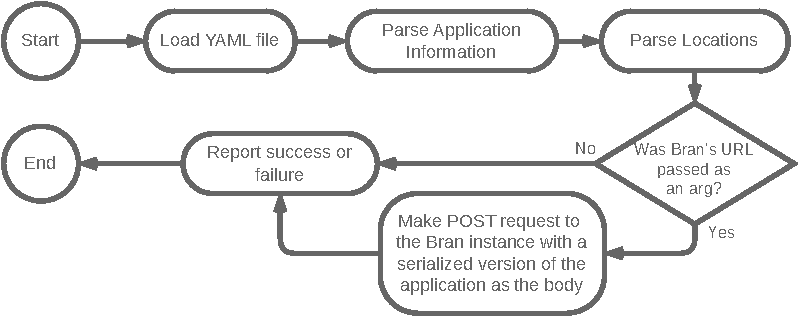
\includegraphics[width=0.9\linewidth]{images/UpdatedLexicalFlow.pdf}
\end{figure}


\subsection{Implementado un Event-Handler}

En el contexto de Smart Campus UIS, cada uno de los mensajes enviados por los dispositivos es manejado como un evento. Es decir, cada mensaje recibido debe ser registrado y procesado por los microservicios de administración para lograr un objetivo final. Este procesamiento, recuerda al patrón de diseño \textit{Observer} en el cual se busca el realizar una acción cada vez que el estado, de lo que se está observando, cambia \cite{Shvets2019}.

Siendo así, se estableció el realizar la implementación de un observador el cual se hará responsable de la captura de los mensajes enviados por los dispositivos y establecer el estado del sistema. De esto, como se puede ver en la figura \ref{fig:procesoLooker} se propuso un proceso que debía realizar el observador, apodado \textit{Looker}, a implementar.

\begin{figure}[ht]
    \caption{\\Primera propuesta del proceso a realizar por \textit{Looker}} 
    \centering
    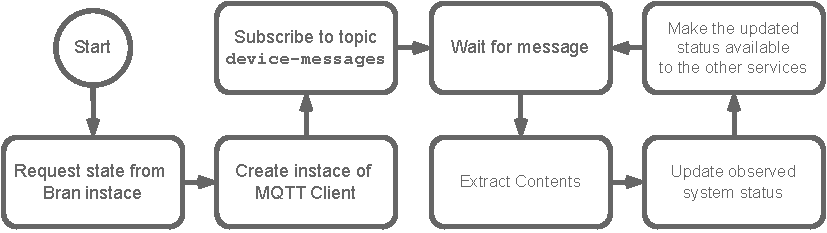
\includegraphics[width=\linewidth]{images/LookerProcess.pdf}
    \label{fig:procesoLooker}
\end{figure} 

Este primer acercamiento, es bastante directo en cuanto a la implementación a realizar. Tras adquirir la definición del estado objetivo, se inicializa un cliente de MQTT, conectado el broker usado por Smart Campus UIS y subscrito al tópico usado por los dispositivos, \texttt{device-messages} \cite{SmartCampusGithub}, este empezaría a procesar los mensajes a medida que estos van llegando. 

Cada mensaje recibido se somete a un conjunto de pasos para actualizar el estado de la aplicación. La figura \ref{fig:LookerProcessUpdateState} describe el proceso que el observador debe realizar con el fin de procesar los mensajes recibidos, dando como resultado, una versión actualizada del estado de la aplicación. 

\begin{figure}[ht]
    \centering
    \caption{\\Proceso realizado por el observador durante el consumo de los mensajes enviados por los dispositivos} 
    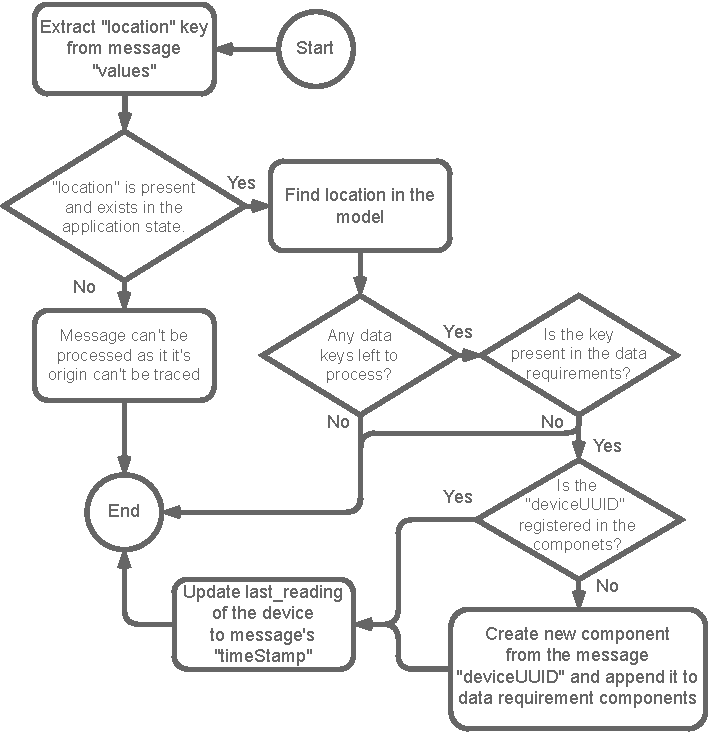
\includegraphics[width=0.70\linewidth]{images/LookerProcessUpdateState.pdf}
    \label{fig:LookerProcessUpdateState}
\end{figure} 

Lo primero a realizar, es ubicarse en el ubicación origen del mensaje. Esto se realiza buscando en las locaciones registradas en la aplicación, usando la llave (Ver figura \ref{fig:jsonSCU}) presente en el mensaje enviado por el dispositivo. En caso que esta, no esté presente, o la locación no haya sido referenciada en la declaración del estado objetivo, el mensaje será descartado. Se debe resaltar que, este puede ser uno de los principales puntos de falla debido a los posibles errores que se puedan presentar al usar nombres diferentes para una locación, sea en los mensajes enviados por problemas en la configuración; o en el momento de la creación del estado de referencia. 

Una vez localizado el origen geográfico del mensaje, se recorrerán los datos reportados por los dispositivos. Estos se cruzarán contra los requerimientos de datos, actualizando los tiempos de los componentes; o registrándolos en caso de que sea el primer mensaje publicado por ellos. Esto se realizará para todas los datos enviados por el dispositivo.
 


\subsection{Comparando Arquitecturas} \label{sec:comparando}

Ahora que se conoce el estado actual del sistema, al igual que estado de referencia; lo siguiente a realizar era la comparación de las arquitecturas. El resultado de esta, daría la base para poder decidir el qué hacer para adaptar el sistema y el cómo hacerlo.

Es necesario definir el como se realizará la evaluación del sistema. Esto no es tan sencillo como hacer una comparación usando un igual (\texttt{A == B}), ya que, el realizar esto, no resultaría realmente información sobre, qué, internamente, presenta problemas.

Ahora, la propiedades implementadas, definidas en los estados objetivo; son la manera las características principales por las cuales es posible realizar la evaluación del sistema. \textit{Timeout}, cumpliendo la función de establecer el tiempo máximo entre los reportes de dispositivos, definiendo cuando estos pueden considerarse como "vencidos"; y \textit{count}, como la cantidad de dispositivos en estado \textit{Coherent} mínima para el desarrollo de la aplicación.

Siendo así, se definió un proceso de comparación consta de evaluar cada componente del sistema en función de las propiedades. A partir de estas, es posible el evaluar el estado de la aplicación. Este proceso es descrito por la figura \ref{fig:LookerProcessClock}.

\begin{figure}[ht]
    \centering
    \caption{\\Proceso reloj realizado por el observador para la actualización del estado de la aplicación} 
    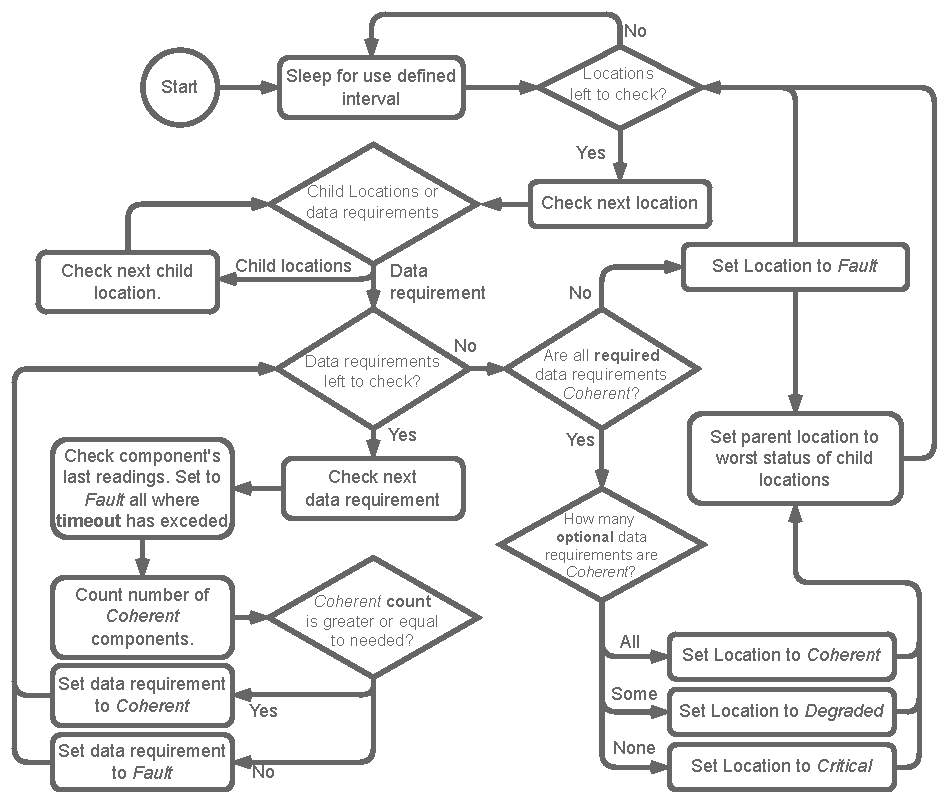
\includegraphics[width=0.85\linewidth]{images/LookerProcessClock.pdf}
    \label{fig:LookerProcessClock}
\end{figure} 

El proceso, apodado reloj, debido a su ejecución dado un intervalo de tiempo definido por el usuario; realiza la evaluación de la aplicación, recorriendo la estructura locación por locación. Siendo así, y con el fin de evitar una dispersión grande de los lugares de procesamiento, se implementó en \textit{Looker}.

Los componentes, pueden existir únicamente en un estado binario, sea \textit{Coherent}, en el caso de que cumplan con las condiciones establecidas en el requerimiento; o \textit{Fault} de lo contrario. Estos se basan únicamente en la propiedad \textit{timeout}, marcándolos de manera correspondiente a partir de su último reporte registrado. 

Así mismo, los requerimientos de datos, con la misma característica de su estado binario; usan propiedad \textit{count} para definir su condición. En caso de que la cantidad total de componentes sea igual a la requerida, se marcará como \textit{Coherent}; de lo contrario, estará en \textit{Fault}. Se ha de resaltar que, debido a que estas propiedades son opcionales durante la declaración, podrán presentarse casos en los que, dada una configuración específica, con un único reporte (o incluso ninguno) estos podrán considerarse válidos durante todo el de ejecución de la aplicación.

Una vez evaluadas los componentes y los requerimientos de datos, lo siguiente es evaluar la locación. Esto dependerá del tipo de la locación. Si es un agrupador, su estado será el peor de los estados de las hijas. De lo contrario, si tiene requerimientos de datos, su estado depende de sus requerimientos de datos y del tipo de cada uno de ellos.

El estado de estas locaciones se determina en dos pasos. En el primer paso, se verifica si alguno de sus requerimientos obligatorios está en estado \textit{Fault}. En ese caso, la locación se considera en estado \textit{Fault}, ya que no puede cumplir con los requisitos mínimos de la aplicación. Para las locaciones sin requerimientos opcionales, este será el final del proceso.

El segundo paso, en el caso de locaciones con requerimientos opcionales, el factor determinante será la cantidad de estados \textit{Coherent}. La locación tendrá un estado \textit{Critical}, \textit{Degraded}, o \textit{Coherent} según si todos, algunos o ninguno de estos requerimientos está en estado \textit{Fault}, respectivamente.

Esta manera de evaluar las locaciones permite el tener una idea más clara del estado de cada una de las locaciones, y por consiguiente, el estado de la aplicación. A partir de esta evaluación, se realizarán las diferentes adaptaciones necesarias con el fin de acercar el estado de la aplicación al estado de referencia esperado.

Una vez actualizado, y evaluado el estado; se tendría que reportar al agregador el nuevo estado de la aplicación. Para esto, se agregó un paso final tras la ejecución del proceso reloj, en la cual, \textit{Looker}, realiza una petición tipo \texttt{PUT} al endpoint designado en \textit{Bran}, con el fin de actualizar el registro. La arquitectura del proyecto, hasta el momento, se puede ver en la figura \ref{fig:StarDuckBasic}.

\begin{figure}[ht]
    \centering
    \caption{\\Arquitectura actual del proyecto}
    \label{fig:StarDuckBasic}
    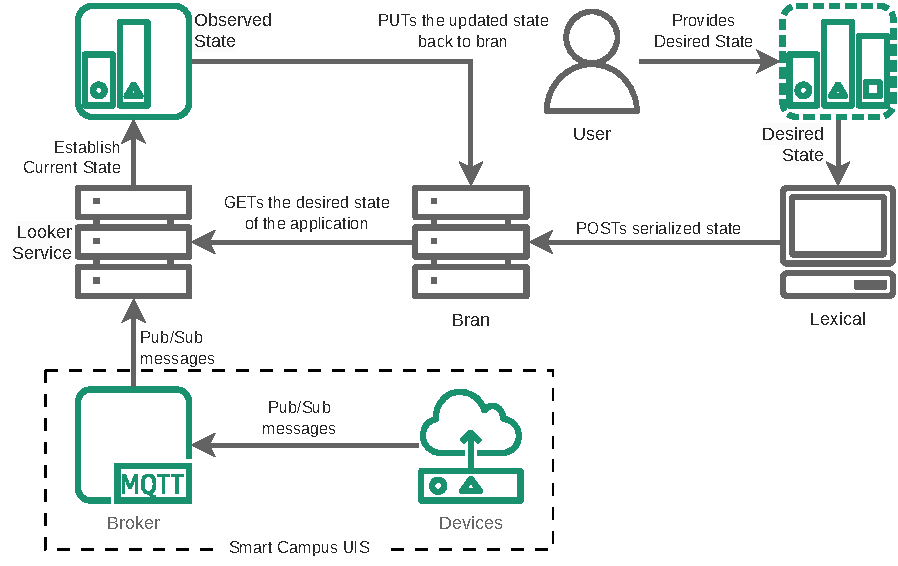
\includegraphics[width=0.8\linewidth]{images/StarDuckBasic.pdf}
\end{figure}





    \section{Adaptando la Arquitectura}

\subsection{Identificando Los Problemas, Estableciendo Acciones}

Ya con una manera de evaluar los estados observados de las aplicaciones definidas, lo siguiente a realizar era el establecer un proceso por el cual se pudieran identificar los problemas en la aplicación, y a partir de esto, establecer las acciones a realizar con el fin de modificar la arquitectura de la aplicación hacia el estado de referencia definido.

Como se estableció durante la sección \ref{sec:comparando}, el estado de la aplicación, en términos generales, es determinada por los estados de sus requerimientos de datos. Siendo así, se definió un proceso por el cual, a partir de las condiciones en las que se encuentren estos requerimientos, se determinen las acciones a realizar con el fin de adaptar la arquitectura.

% \begin{itemize}
%     \item \textbf{\textit{Addition}}: Busca crear nuevos componentes, a partir de servicios, con el fin de cumplir con las necesidades de datos.
%     \item \textbf{\textit{Restart}}: Esta acción está enfocada a reiniciar servicios que puedan haber fallado, con el fin de retornarlos a un estado funcional.
%     \item \textbf{\textit{Reconfigure}}: Busca el realizar cambios en componentes con el fin de cumplir con las necesidades establecidas.
% \end{itemize}

Partiendo de esto, se definió el proceso, descrito por la figura \ref{fig:BranProcess}, en dos partes. La primera, está encargada de la búsqueda e identificación de los problemas dentro de la aplicación; y la segunda, de manera interna, el determinar las acciones a seguir para adaptar la arquitectura. 

\begin{figure}[ht]
    \centering
    \caption{\\Proceso para la identificación de problemas de los requerimientos de datos}
    \label{fig:BranProcess}
    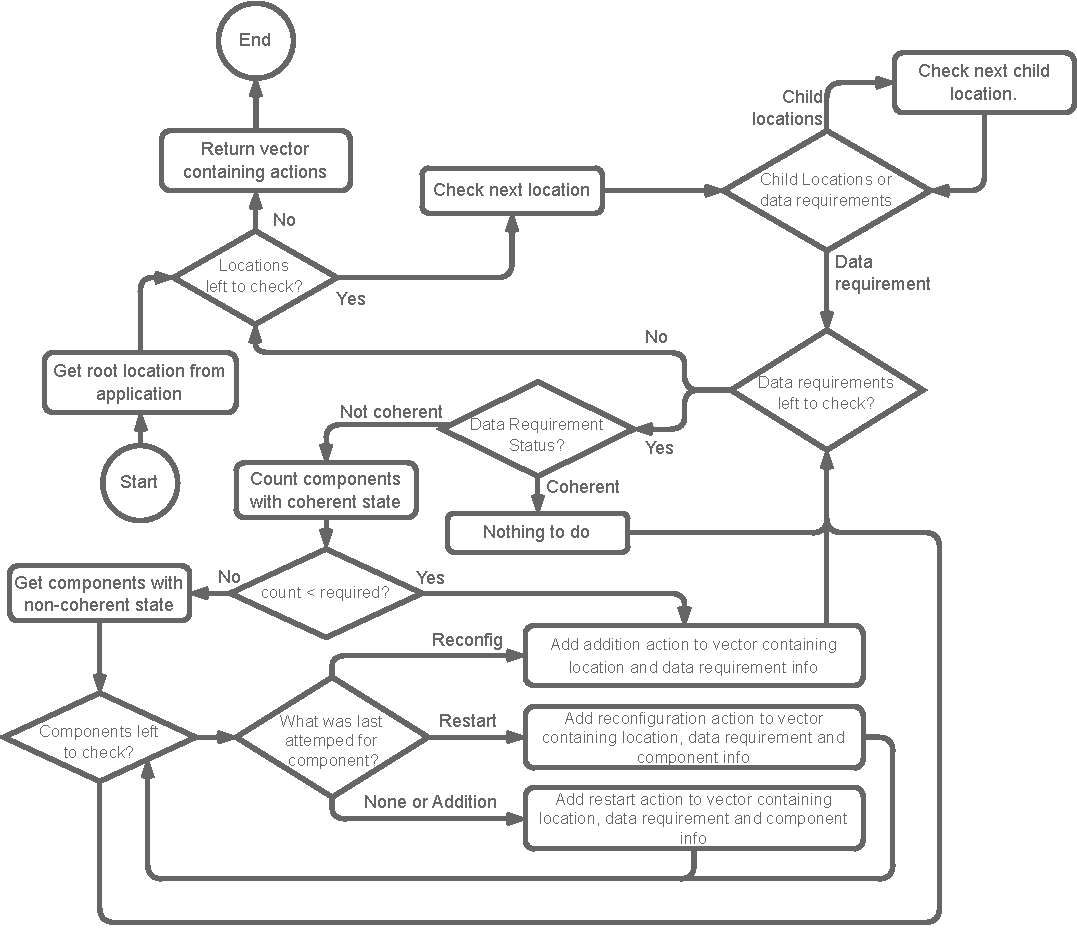
\includegraphics[width=0.9\linewidth]{images/BranProcessPlanner.pdf}
\end{figure}

La manera en la de que se identifican los problemas es similar a la vista en la figura \ref{fig:LookerProcessClock}. Se recorren las locaciones, buscando requerimientos de datos. Una vez en una de estas locaciones, se validan los requerimientos y se definen las acciones.

Ahora, las posibles acciones a tomar para la arquitectura de la aplicación, como se vió durante la sección \ref{sec:MecAdap}, dependen de los objetivos y los requerimientos del sistema. Siendo así, se tomaron 3 tipos de acciones por las cuales se puede modificar el estado del sistema: \textit{Addition}, \textit{Restart} y \textit{Reconfigure}.

Todos los requerimientos en un estado diferente a \textit{Coherent}, son evaluados con el fin de establecer la acción a realizar. Lo primero, es revisar la cantidad de componentes registrados en el requerimiento; si se tiene menos de los requeridos, se realizará un acción tipo \textit{Addition} con el fin de cumplir con el numero de fuentes de datos esperada.

En el caso de tener la cantidad requerida de dispositivos, pero estado aún en estado \textit{Fault}; la siguiente opción es reiniciar el servicio. Esto busca poner nuevamente en un estado válido el componente, en caso de que haya quedado en un estado inválido; o poner nuevamente en ejecución el servicio en el escenario de que este haya muerto.

Si el reiniciar no tiene efecto en el estado del componente, la siguiente opción es reconfigurar el componente. Esto busca la modificación de algún aspecto, sea la actualización una variable de ambiente o parámetro, con el fin de retornarlo a un estado válido. 
 
Finalmente, si todo falla y no es posible recuperar el dispositivo; la última opción es iniciar un nuevo servicio el cual pueda suplir las condiciones de su predecesor. De esta manera, aún es posible retornar la aplicación hacia un estado válido, independiente de los componentes en un estado irrecuperable.

La implementación de este proceso, se realizó en el agregador \textit{Bran}. Esto debido a que, al tener el estado de las aplicaciones, cortesía de lo observado por \textit{Looker}; deja a este servicio como el punto medio de la aplicación, encargado de definir las acciones a realizar.

\subsection{De Acciones, a Instrucciones}

Ahora, se tienen las acciones a realizar para poder adaptar la arquitectura de la aplicación hacia el estado de referencia; sin embargo, estas acciones no contienen la información necesaria para ejecutar ninguno de los procesos necesarios.

Partiendo de esto, se determinó la necesidad de una colección estructuras de datos, que contuvieran las instrucciones a seguir, para cada una de las acciones definidas. Esta, debe especificar la locación de la aplicación en la cual se ejecutan, con el fin de tener una mejor granularidad y control sobre la manera en la que se realizan las modificaciones en la arquitectura.

En consecuencia, como se observa en la figura \ref{fig:Directives}, se definió una estructura de datos llamada \texttt{Directive}. Esta contiene tres campos adicionales para las estructuras \texttt{AdditionOrder}, \texttt{RestartOrder}, y \texttt{ReconfigureOrder}; que corresponden con las acciones \textit{Addition}, \textit{Restart} y \textit{Reconfigure}, respectivamente.

\begin{figure}[ht]
    \centering
    \caption{\\UML de la estructura de directivas y ordenes}
    \label{fig:Directives}
    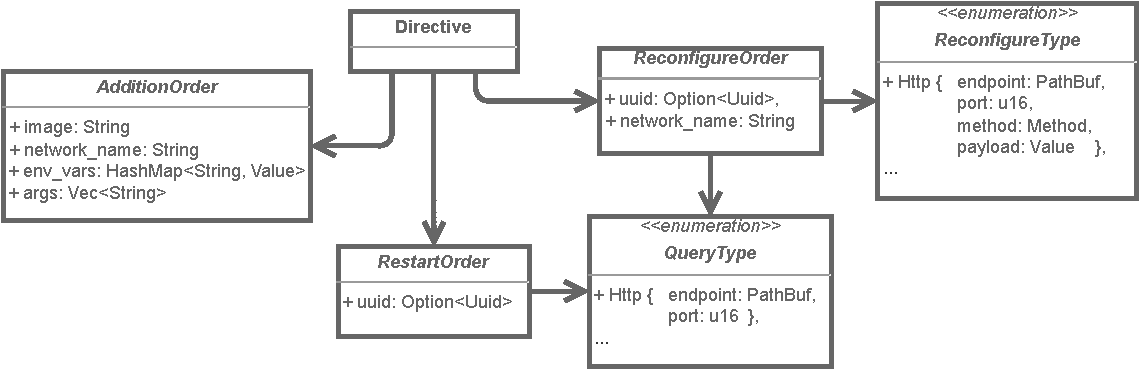
\includegraphics[width=0.85\linewidth]{images/Directives.pdf}
\end{figure}

Cada una estas directivas, y ordenes, se agregan a un registro en \textit{Bran}, usando el nombre de la aplicación y la locación a la pertenecen para su indexación. Cada una se registra usando un endpoint dedicado a la recepción de las órdenes.

La orden de adición contiene el nombre de la imagen del servicio a desplegar, la red a la cual debe conectarse para poder interactuar con los demás servicios, y los argumentos que se deben pasar sea como variables de ambiente o argumentos de línea de comando. 

Las órdenes de reinicio y reconfiguración poseen el \textit{UUID} del dispositivo que buscan afectar. Siendo así, al ser necesario tener una manera por la cual identificar qué servicio es qué componente, se implementó el enum \texttt{QueryType}. Este, contiene la información de como debe buscarse el contenedor en la red. Para esta primera implementación, su única variante es una búsqueda \textit{Http} hacia un endpoint y un puerto.

Finalmente, la orden de reconfiguración tiene como parte extra la red en la que se buscara el servicio a reiniciar y el tipo de reconfiguración (\texttt{ReconfigureType}) a realizar. Este funciona de manera similar a QueryType, en tanto indica la manera en la que se aplicará la reconfiguración. En este caso, para la variante \textit{Http} implementada, indica el endpoint y el puerto a usar, junto con el método y payload que deben ir en la petición para hacer la reconfiguración efectiva.

Se ha de resaltar que, estas ordenes, aunque contienen las instrucciones para poder realizar modificaciones a la arquitectura, en el momento de su declaración, no están completas y requieren de información extra para poder ejecutarse.

El proceso de la figura \ref{fig:BranExecution}, muestra el proceso por el cual las órdenes presentes en el registro de directivas de \textit{Bran}, son usadas como base para la construcción de las órdenes finales, y son enviadas para su posterior ejecución.

\begin{figure}[ht]
    \centering
    \caption{\\Proceso de decisión de acciones base realizado por Bran}
    \label{fig:BranExecution}
    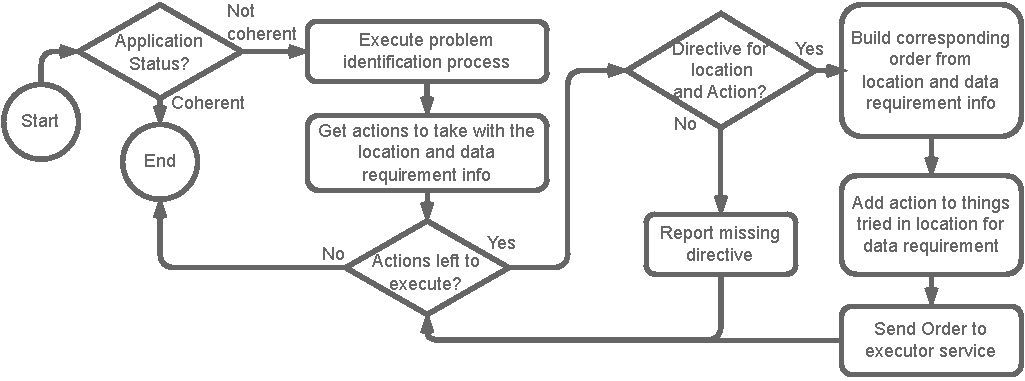
\includegraphics[width=0.9\linewidth]{images/BranProcessExecuter.pdf}
\end{figure}

Su ejecución inicia validando el estado de la aplicación reportada. En caso de este sea diferente a \textit{Coherent}, se llamará al proceso de identificación de problemas para obtener las acciones a realizar para alterar el estado de aplicación.

Una vez recibido el vector conteniendo las acciones, y la información asociada correspondiente, se realizará la construcción de cada una de las órdenes a ejecutar. Esta construcción se realiza a partir de las instrucciones bases establecidas en las directivas usando el UUID para las acciones de \textit{Restart} y \textit{Reconfigure}; y la información de la locación y el requerimiento de dato en las acciones de \textit{Addition}\footnote{Es necesario resaltar que estas construcciones, en especial para el caso de las acciones de \textit{Addition}, fueron implementadas para funcionar con los servicios \textit{Mocker} desarrollados específicamente para el proyecto. Esto se explorará más a fondo durante la sección \ref{sec:experimental} y \ref{sec:future}.}. 

Ya con las ordenes creadas, estas se enviaran al servicio encargado de ejecutar las instrucciones, dando como como resultado, modificaciones en la arquitectura.


\subsection{De Instrucciones a Acciones}

% Se estableció tener un servicio aparte para la ejecución de las ordenes. Esto se debe a las condiciones especiales que debe tener el encargado de realizar el paso final en el ciclo MAPE-K (Ver figura \ref{fig:mapek}). 

% Smart Campus UIS, como plataforma, se ejecuta sobre contenedores de docker; y para efectos de esta primera versión del proyecto, toda la arquitectura de presente, se ejecuta sobre contenedores. Siendo así, la característica principal que debe tener nuestro ejecutor, es la posibilidad de comunicarse con los diferentes contenedores.

% Esto se realizó a partir de 

Ya con las instrucciones necesarias para poder realizar cambios en la arquitectura de las aplicaciones, se realizó la implementación de un servicio encargado de ejecutar las ordenes recibidas desde \textit{Bran}.

Ahora, Smart Campus UIS, como plataforma, se ejecuta sobre contenedores de docker; y para efectos de esta primera versión del proyecto, toda la arquitectura de presente, se ejecuta sobre contenedores. Como consecuencia, era necesario que el servicio implementado, tuviera la de ejecutar comandos de docker con el fin de poder llevar a cabo las acciones.

Esto se solucionó usando la Docker Engine API como el canal de comunicación entre el servicio, y el resto de la arquitectura. Esto se debe a que, esta API REST, permite la interacción directa con el daemon de Docker \cite{docker}, posibilitando la ejecución de todos los comandos relacionados con docker, desde el iniciar y detener servicios hasta crear y eliminar contenedores.

El servicio, apodado \textit{DoThing}, realiza visto en la figura \ref{fig:DoThing}. Este está orientado principalmente al procesamiento de las peticiones realizadas, por lo que es relativamente sencillo en cuanto a las acciones que este realiza. 

\begin{figure}[ht]
    \centering
    \caption{\\Proceso base de DoThing}
    \label{fig:DoThing}
    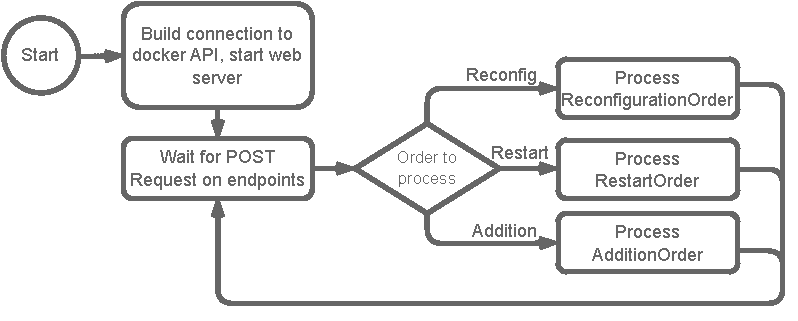
\includegraphics[width=0.75\linewidth]{images/DoThingProcess.pdf}
\end{figure}

Tras inicializar la conexión con la API de Docker, iniciará un servidor web por el cual estará recibiendo las órdenes a ejecutar. Cada tipo de acción tiene su propio endpoint donde se realiza un proceso específico para poder ejecutarla. Cada acción realizada, registrará los contenedores afectados en un registro interno, con el fin de facilitar el procesamiento de múltiples acciones sobre un servicio. 

Las ordenes de \textit{Addition}, como se referencia en la figura \ref{fig:DoThingAddition}, realizan el proceso a partir de la \texttt{image}, \texttt{env\_vars} y \texttt{args}, declarados en la orden, para construir el contenedor con su respectivo servicio.

\begin{figure}[ht]
    \centering
    \caption{\\Proceso para la ejecución de ordenes de adición}
    \label{fig:DoThingAddition}
    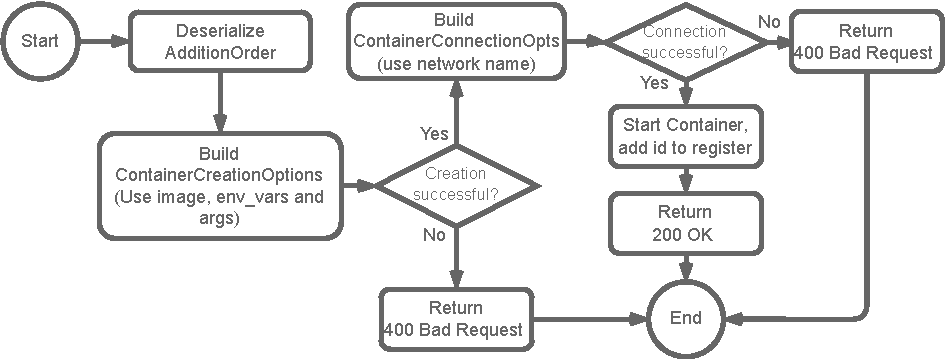
\includegraphics[width=0.8\linewidth]{images/DoThingAddition.pdf}
\end{figure}

Una vez se tenga el contenedor creado, usando \texttt{network\_name}, se conectará el contenedor creado a la red indicada. De no presentarse errores durante este proceso, se iniciará el contenedor, se agrega al registro y retorna \texttt{200 OK}. 

Las órdenes de tipo \textit{Restart}, referenciadas en la figura \ref{fig:DoThingRestart} pueden ejecutarse de una de dos maneras, dependiendo del estado del servicio a afectar. 

\begin{figure}[ht]
    \centering
    \caption{\\Proceso para la ejecución de ordenes de reinicio}
    \label{fig:DoThingRestart}
    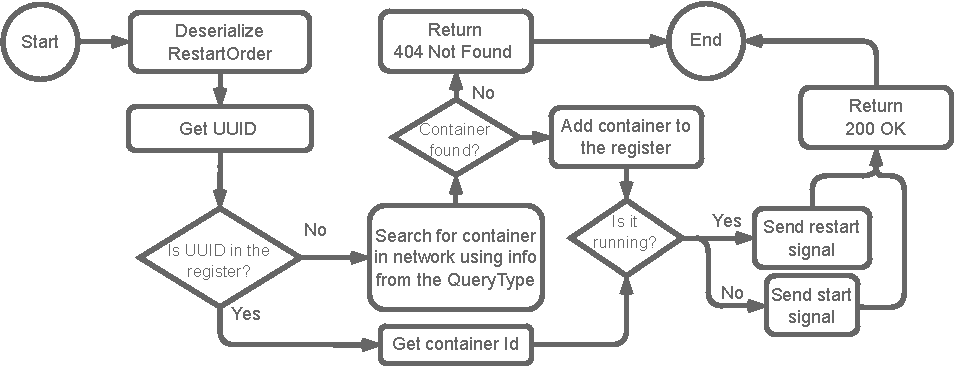
\includegraphics[width=0.9\linewidth]{images/DoThingRestart.pdf}
\end{figure}

Primero, se realiza la búsqueda del contenedor en el registro; de no estar presente, se realizará la búsqueda de este usando la información proveída en el \textit{QueryType} de la orden.

Una vez identificado el servicio, si está corriendo\footnote{Referido en la documentación de \href{https://docs.docker.com/engine/api/v1.43/\#tag/Container/operation/ContainerInspect}{Docker Engine API} como \textit{Running}}, la orden de reinicio será equivalente al comando \texttt{docker restart <container>}, esto con el objetivo de eliminar \textit{cuelgues} en el servicio. Por el contrario, si el contenedor no está en ejecución, la orden ejecutará el equivalente al comando \texttt{docker start <container>}, para así iniciar nuevamente el servicio.

Finalmente, las órdenes de tipo \textit{Reconfigure}, cuyo proceso puede verse en la figura \ref{fig:DoThingReconfig}, es similar al realizado para las órdenes de tipo \textit{Restart}. 

\begin{figure}[ht]
    \centering
    \caption{\\Proceso para la ejecución de ordenes de reconfiguración}
    \label{fig:DoThingReconfig}
    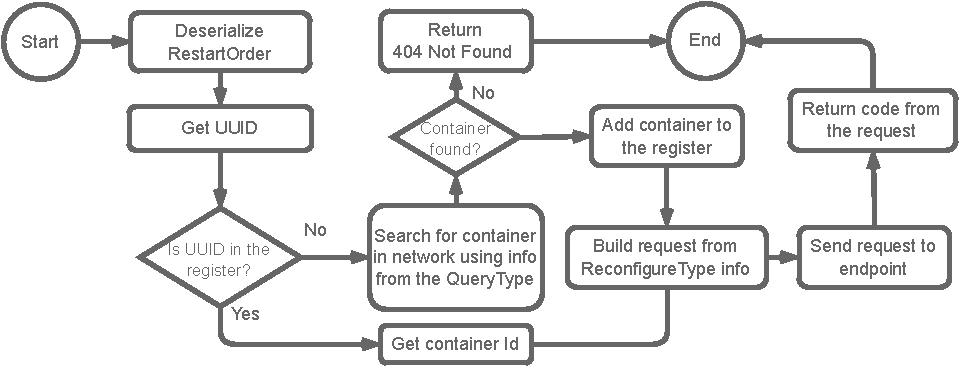
\includegraphics[width=0.8\linewidth]{images/DoThingReconfig.pdf}
\end{figure}

Una vez ubicado el servicio, se construirá, a partir de los datos reportados en \textit{ReconfigureType}, la petición a realizar en el servicio. Esta, en consecuencia, se enviará usando un cliente \textit{Http} y esperará a la respuesta de esta. El resultado, de esta transacción, será el mismo reportado por \textit{DoThing} hacia \textit{Bran}.

Ahora, con la implementación de este servicio, encargado de ejecutar las acciones requeridas para la adaptación de las arquitecturas de las aplicaciones, completa el ciclo autonómico MAPE-K implementado para Smart Campus UIS. 

Una vez ejecutadas las órdenes; el efecto de estas, serían captadas por el observador, evaluando nuevamente el estado de la aplicación, e, idealmente, reportando un cambio positivo hacia la coherencia esperada con el estado de referencia definido en un principio.

La arquitectura final del presente proyecto, con toda la implementación de los servicios, puede ver se en la figura \ref{fig:StarDuckFinal}.


\begin{figure}[ht]
    \centering
    \caption{\\Arquitectura completa del proyecto}
    \label{fig:StarDuckFinal}
    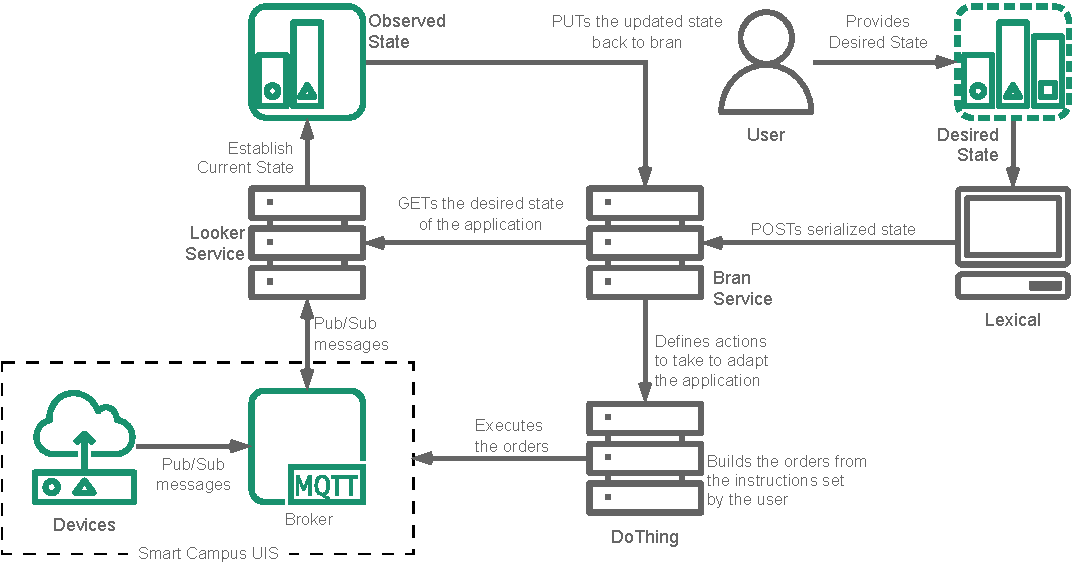
\includegraphics[width=\linewidth]{images/StarDuckFinal.pdf}
\end{figure}



    \section{Validación de la Implementación} \label{sec:experimental}

Lo último a realizar fue la validación de las funcionalidades de la aplicación desarrollada. Para ello, se establecieron escenarios de prueba por los cuales se pueda comprobar el funcionamiento de aplicación. Estos, se definieron con el fin de probar la capacidad y la efectividad de los mecanismos implementados de modificar el estado inicial de la aplicación hacia el estado de referencia, al igual que la identificación de algunas de las falencias de esta.

Ahora, se debe resaltar que, las pruebas se realizaron usando un servicio genérico, apodado Mocker, encargado de la generación de datos, especialmente desarrollado para funcionar en condiciones ideales. 

Para cada una de estas pruebas, se definió un estado de referencia, dadas unas condiciones iniciales, y una serie de eventos los cuales modificarán nuevamente el estado de la aplicación, las cuales tendrán que ser nuevamente manejadas.

\subsection{Resultados De Escenario Experimental A}

El objetivo de las pruebas realizadas en el presente escenario experimental, era validar que, los procesos implementados, efectivamente realizaran la adaptación de las aplicaciones desde un estado de completa falla, en donde ninguno de los datos necesarios estuviera presente.

Siguiendo los pasos definidos en la sección \ref{sec:EscenarioExperimentalA}, se realizó el despliegue de los servicios base de Smart Campus UIS, al igual que \textit{Bran} y \textit{DoThing}. Como se presenta en la figura \ref{fig:LookerStart}, se registró el estado de referencia al agregador tras validarlo usando \textit{Lexical}, y se fijaron las directivas a usar para la adaptación de la arquitectura.

\begin{figure}[ht]
    \centering
    \caption{\\Aplicación y directivas registradas en Bran}
    \label{fig:BranStart}
    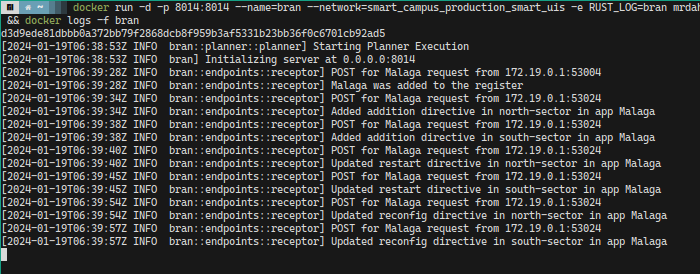
\includegraphics[width=0.9\linewidth]{images/BranStart.png}
    \vspace{-4mm}
\end{figure}

Una vez se inició el servicio \textit{Looker}, como se ve en la figura \ref{fig:LookerStart}, este empezó a evaluar el estado de la aplicación; que al no tener ningún tipo de reporte de algún componente, entró directamente en estado de falla. 

\begin{figure}[ht]
    \centering
    \caption{\\Looker evalúa el estado de la aplicación}
    \label{fig:LookerStart}
    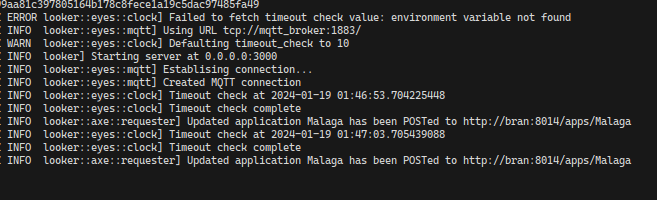
\includegraphics[width=0.9\linewidth]{images/LookerStart.png}
    \vspace{-4mm}
\end{figure}

El estado observado, se reportó a \textit{Bran}, el cual, realizó el recorrido para identificar los puntos de falla de la aplicación. Como se observa en la figura \ref{fig:BranPlan}, como era de esperar, los tres requerimientos definidos en cada una de las locaciones estaba en estado de falla. Al no haber componentes reportando datos, como era de esperarse, se definieron acciones \textit{Addition} para todos los componentes de la aplicación. 

\begin{figure}[ht]
    \centering
    \caption{\\Bran identifica los problemas y establece las acciones}
    \label{fig:BranPlan}
    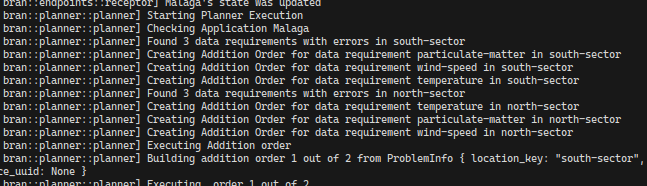
\includegraphics[width=0.9\linewidth]{images/BranPlanning.png}
    \vspace{-4mm}
\end{figure}

A partir de las acciones, se crearon las órdenes para ejecución usando las directivas como base. Como se puede ver en la figura \ref{fig:DoThingDoing}, cada una de estas se envió a \textit{DoThing}, el cual realizó el procesamiento requerido para la construcción y arranque de los contenedores. El resultado de este procesamiento se puede ver en la figura \ref{fig:ContainerState}

\begin{figure}[ht]
    \centering
    \caption{\\DoThing ejecuta las acciones establecidas por Bran }
    \label{fig:DoThingDoing}
    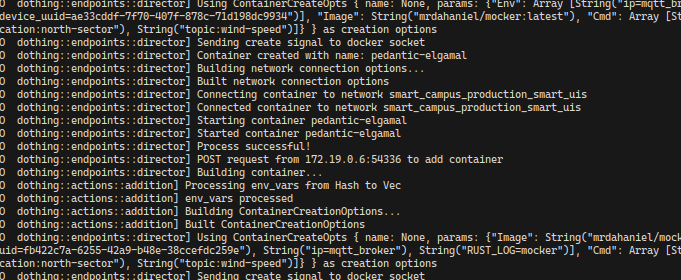
\includegraphics[width=0.9\linewidth]{images/DoThingDoing.png}
    \vspace{-4mm}
\end{figure}

\begin{figure}[ht]
    \centering
    \caption{\\Contenedores creados por DoThing en respuesta a las órdenes recibidas}
    \label{fig:ContainerState}
    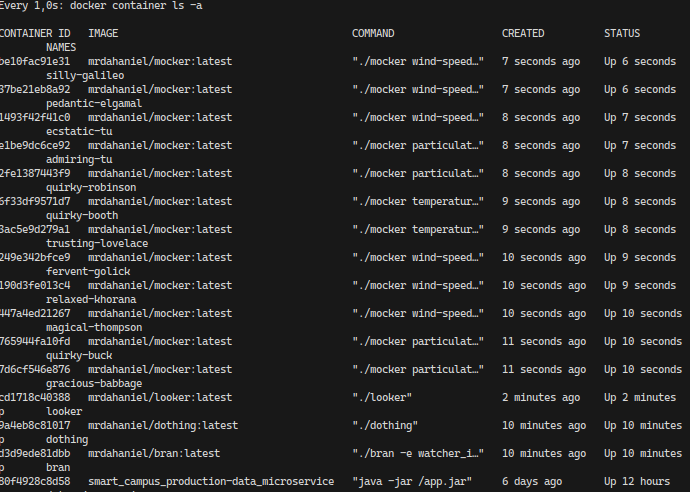
\includegraphics[width=0.9\linewidth]{images/ContainerLaunching.png}
    \vspace{-4mm}
\end{figure}

En total, se crearon 12 contenedores, que corresponden a los 12 componentes requeridos para el desarrollo de la aplicación. Cada uno de ellos configurado para suplir las necesidades de operación establecidas en el estado de referencia. Estos despliegues, como era de esperarse, fueron detectado por \textit{looker}, el cual realizó el nuevas valoraciones del estado. 

Los valores por defecto de los servicios usados para estas pruebas es un intervalo de tiempo entre mensajes de un minuto. Este valor por defecto, aunque para los requerimientos de datos cuyos \textit{timeout}, sean superiores, supliría las necesidades de la aplicación. Sin embargo, en el marco de esta simulación, esta frecuencia de reportes no es suficiente para cumplir con el estado de referencia de los requerimiento de temperatura de las locaciones.

Como consecuencia, el estado de la aplicación regresó a estado \textit{Fault}, y \textit{Bran}, al detectar los problemas, emitió las acciones tipo \textit{Restart} con el fin de traer los contenedores a un estado válido. Esto se puede ver en la figura \ref{fig:BranPlan2}.

\begin{figure}[H]
    \centering
    \caption{\\Bran identifica otros problemas en la aplicación}
    \label{fig:BranPlan2}
    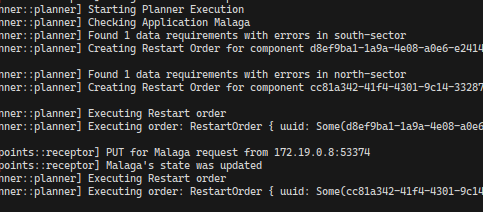
\includegraphics[width=0.9\linewidth]{images/BranRestarting.png}
    \vspace{-4mm}
\end{figure}

Este intento de reiniciar los servicios, como era de esperarse, no fue realmente efectiva debido a que la falla se debe a un problema en la configuración del servicio. Siendo así, la aplicación se mantuvo en estado de falla. Se esperaba que, ambos componentes encargados de la temperatura, al ya haber descartado el reinicio como un mecanismo efectivo para esta situación, fueran sometidos a una acción de reconfiguración, sin embargo, como se observa en la figura \ref{fig:BranPlan3}, en ese instante, sólo el componente de \texttt{north-sector} fue afectado.

\begin{figure}[ht]
    \centering
    \caption{\\Bran establece acciones de reconfiguración para adaptar la aplicación}
    \label{fig:BranPlan3}
    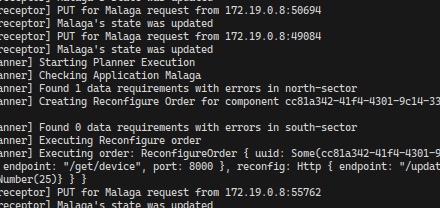
\includegraphics[width=0.9\linewidth]{images/BranReconfiguring.png}
    \vspace{-4mm}
\end{figure}

Esta reconfiguración fue ejecutada por \textit{DoThing}, y tomó efecto, alterando el valor por defecto entre mensajes, pasando de un reporte cada minuto, a uno cada 25 segundos\footnote{Según lo definido en las directivas presentes en el apéndice \ref{ape:DirectivesA}}. Con el nuevo valor, los componentes de temperatura, empezaban a reportar con mayor frecuencia, cumpliendo con las expectativas.

Poco tiempo después, el componente de temperatura de \texttt{south-sector}, reportó el estado de falla, por lo se ejecutó la misma acción de reconfiguración que con el componente de la otra locación, llevando el estado de la aplicación a \textit{Coherent}.

A partir de esta simulación, se pudo validar que el proceso implementado, tiene la capacidad de realizar la adaptación desde el peor escenario, hacia un esto de coherencia con la aplicación declarada inicialmente. Todas las acciones definidas por \textit{Bran}, permitieron modificar el estado de manera positiva.

Sin embargo, se identificaron algunas limitaciones de esta implementación. Como se observa en la figura \ref{fig:BranPlan3}, se muestra que \texttt{south-sector} no presenta problemas en sus requerimientos, cuando, debido a su configuración, debía estar en estado de falla. 

Esto se debe a un \textit{quirk} de la implementación realizada. Al manejar los procesos cada cierto intervalo de tiempo, es posible que un componente se encuentren en estado de falla, pero alcance a pasar a coherente justo antes de la evaluación de las acciones a tomar. Eventualmente, el componente fallaría en reportar antes de una una de las evaluaciones desencadenando en una acción, como fue el caso con la tardía reconfiguración del componente de \texttt{south-sector}. 

\subsection{Resultados De Escenario Experimental B}

El objetivo principal del escenario experimental B, era evaluar la capacidad de la implementación realizada de recuperar una aplicación en estado de coherencia, en donde se presenta una falla masiva, nuevamente a un estado válido; al igual que la capacidad de Bran de manejar más de una aplicación, como se había nombrado en la sección \ref{sec:Centering}.

Igual que durante el escenario experimental A, se realizó el despliegue de los servicios \textit{Bran} y \textit{DoThing}. Como se observa en la figura \ref{fig:Bran2Apps}, se definieron las arquitecturas objetivo de las dos aplicaciones a monitorear, al igual que las directivas a usar durante este proceso.

\begin{figure}[ht]
    \centering
    \caption{\\Aplicaciones y directivas registradas en Bran}
    \label{fig:Bran2Apps}
    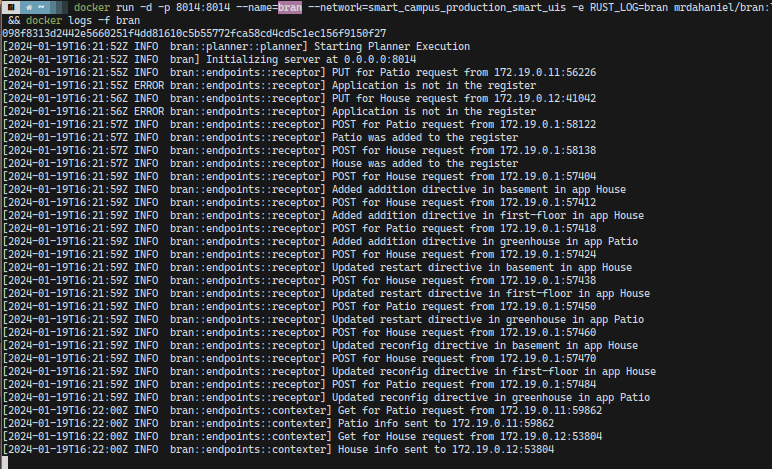
\includegraphics[width=0.9\linewidth]{images/BranBScenarioDeclarition.png}
    \vspace{-4mm}
\end{figure}

Seguidamente, como se observa en la figura \ref{fig:Looker2Apps}, se desplegaron los servicios de \textit{Looker} para cada una de las aplicaciones a monitorear. Ya con esta base lista, y como se definió en los pasos a seguir, se desplegaron de manera manual, un total de 3 servicios \textit{Mocker} con configuraciones específicas (tanto de los datos que estos reportaban, como de los tiempos de reporte) con el fin de cumplir con los requerimientos de datos definidos para las dos aplicaciones. 

\begin{figure}[H]
    \centering
    \caption{\\Dos instancias de looker monitoreando las aplicaciones declaradas}
    \label{fig:Looker2Apps}
    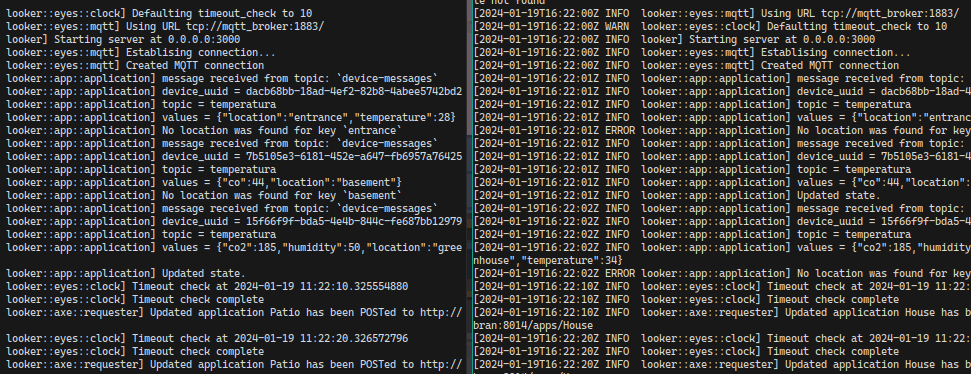
\includegraphics[width=0.9\linewidth]{images/Looker2Apps.png}
    \vspace{-4mm}
\end{figure}

Como era de esperarse, con las configuraciones hechas a la medida de las aplicaciones, el estado de estas era \textit{Coherent}, sin la necesidad de ningún tipo de cambios en los dispositivos. Siendo así, como se ve en la figura \ref{fig:KillThemAll}, se matan los 3 contenedores desplegados, y se elimina uno de ellos.

\begin{figure}[H]
    \centering
    \caption{\\Se matan los contenedores con los servicios iniciales}
    \label{fig:KillThemAll}
    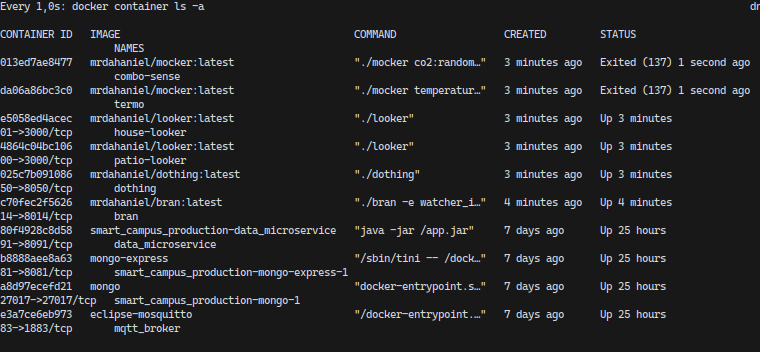
\includegraphics[width=0.9\linewidth]{images/Killing.png}
    \vspace{-4mm}
\end{figure}

La figura \ref{fig:FindAny}, muestra el como \textit{Bran}, define las órdenes para reiniciar los servicios para traer la aplicación a un estado nuevamente. En condiciones normales, se esperaría que esto sea lo único a realizar para adaptar la arquitectura, sin embargo, este no fue el caso.

\begin{figure}[ht]
    \centering
    \caption{\\Bran intenta reiniciar los contenedores}
    \label{fig:FindAny}
    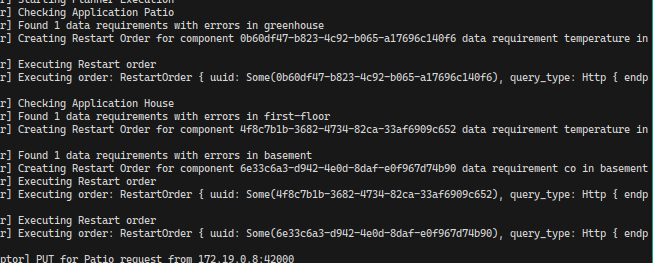
\includegraphics[width=0.9\linewidth]{images/BranOrdersRestarts.png}
    \vspace{-4mm}
\end{figure}

\newpage

Ya que los contenedores no fueron desplegados, o ha sido modificados, de ninguna manera por \textit{DoThing}, no estos no están mapeados. Siendo así, como se ve en la figura \ref{fig:CantFindAny}, es necesario buscar los contenedores en la red, pero, al estar los servicios muertos, y depender de la consulta \textit{Http} para poder identificarlos, no puede encontrarlos.


\begin{figure}[ht]
    \centering
    \caption{\\DoThing no puede encontrar los contenedores}
    \label{fig:CantFindAny}
    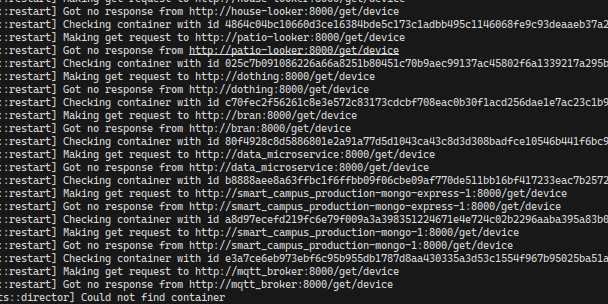
\includegraphics[width=0.9\linewidth]{images/CantFind.png}
    \vspace{-4mm}
\end{figure}

Esto demuestra otra de las falencias con la implementación realizada, que es la búsqueda del crecimiento de la fase de conocimiento. El haber identificado los componentes, antes de que se presentaran problemas, hubiera posibilitado la ejecución de órdenes cuando los servicios estén caídos. Así mismo, se hubiera podido establecer una búsqueda que no dependiera del estado de los componentes, quizás usando tags.

El resultado final, es que \textit{Bran}, al no poder actuar de otra manera, como se observa en la figura \ref{fig:HadToAdd}, ordena acciones de adición para suplir los componentes. Esto, eventualmente, resulta en el regreso de la aplicación a un estado válido, pero sigue sin ser lo ideal.

\begin{figure}[ht]
    \centering
    \caption{\\Bran crea órdenes de adicción}
    \label{fig:HadToAdd}
    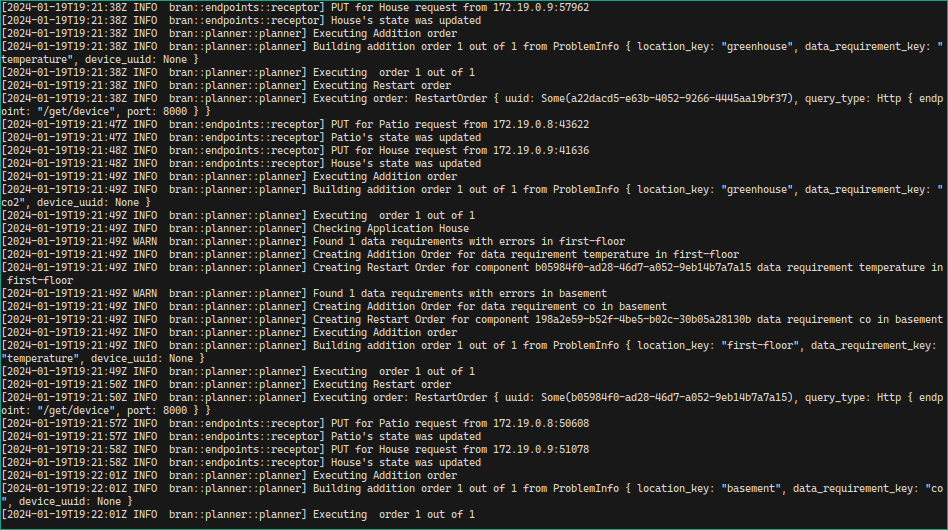
\includegraphics[width=0.9\linewidth]{images/ReLaunchIT.png}
    \vspace{-4mm}
\end{figure}
    
    \section{\ Análisis de Resultados}

\subsection{Resultados De Escenario Experimental A}

El objetivo de las pruebas realizadas en el presente escenario experimental, era validar que, los procesos implementados, efectivamente realizaran la adaptación de las aplicaciones desde un estado de completa falla, en donde ninguno de los datos necesarios estuviera presente.

Siguiendo los pasos definidos en la sección \ref{sec:EscenarioExperimentalA}, se realizó el despliegue de los servicios base de Smart Campus UIS, al igual que \textit{Bran} y \textit{DoThing}. Como se presenta en la figura \ref{fig:LookerStart}, se registró el estado de referencia al agregador tras validarlo usando \textit{Lexical}, y se fijaron las directivas a usar para la adaptación de la arquitectura.

\begin{figure}[ht]
    \centering
    \caption{\\Aplicación y directivas registradas en Bran}
    \label{fig:BranStart}
    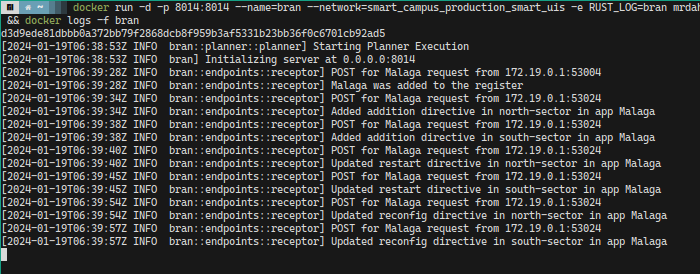
\includegraphics[width=0.9\linewidth]{images/BranStart.png}
    \vspace{-4mm}
\end{figure}

Una vez se inició el servicio \textit{Looker}, como se ve en la figura \ref{fig:LookerStart}, este empezó a evaluar el estado de la aplicación; que al no tener ningún tipo de reporte de algún componente, entró directamente en estado de falla. 

\begin{figure}[ht]
    \centering
    \caption{\\Looker evalúa el estado de la aplicación}
    \label{fig:LookerStart}
    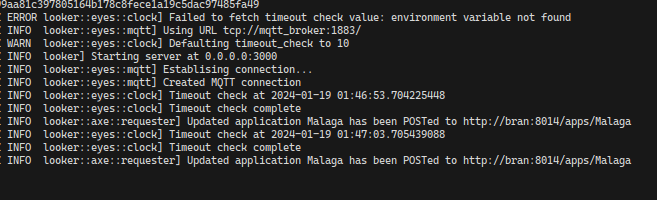
\includegraphics[width=0.9\linewidth]{images/LookerStart.png}
    \vspace{-4mm}
\end{figure}

El estado observado, se reportó a \textit{Bran}, el cual, realizó el recorrido para identificar los puntos de falla de la aplicación. Como se observa en la figura \ref{fig:BranPlan}, como era de esperar, los tres requerimientos definidos en cada una de las locaciones estaba en estado de falla. Al no haber componentes reportando datos, como era de esperarse, se definieron acciones \textit{Addition} para todos los componentes de la aplicación. 

\begin{figure}[ht]
    \centering
    \caption{\\Bran identifica los problemas y establece las acciones}
    \label{fig:BranPlan}
    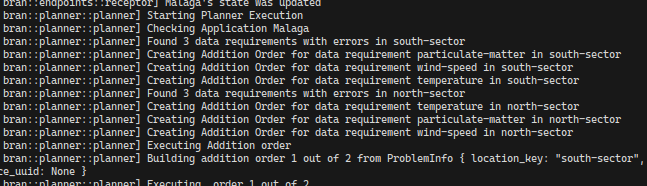
\includegraphics[width=0.9\linewidth]{images/BranPlanning.png}
    \vspace{-4mm}
\end{figure}

A partir de las acciones, se crearon las órdenes para ejecución usando las directivas como base. Como se puede ver en la figura \ref{fig:DoThingDoing}, cada una de estas se envió a \textit{DoThing}, el cual realizó el procesamiento requerido para la construcción y arranque de los contenedores. El resultado de este procesamiento se puede ver en la figura \ref{fig:ContainerState}

\begin{figure}[ht]
    \centering
    \caption{\\DoThing ejecuta las acciones establecidas por Bran }
    \label{fig:DoThingDoing}
    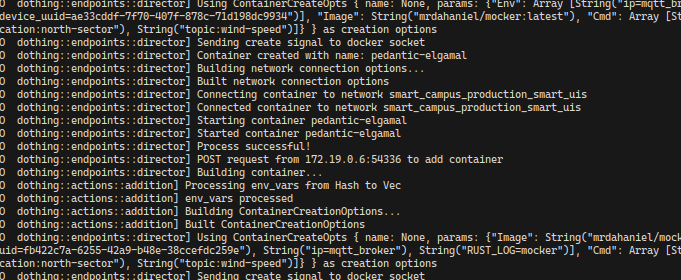
\includegraphics[width=0.9\linewidth]{images/DoThingDoing.png}
    \vspace{-4mm}
\end{figure}

\begin{figure}[ht]
    \centering
    \caption{\\Contenedores creados por DoThing en respuesta a las órdenes recibidas}
    \label{fig:ContainerState}
    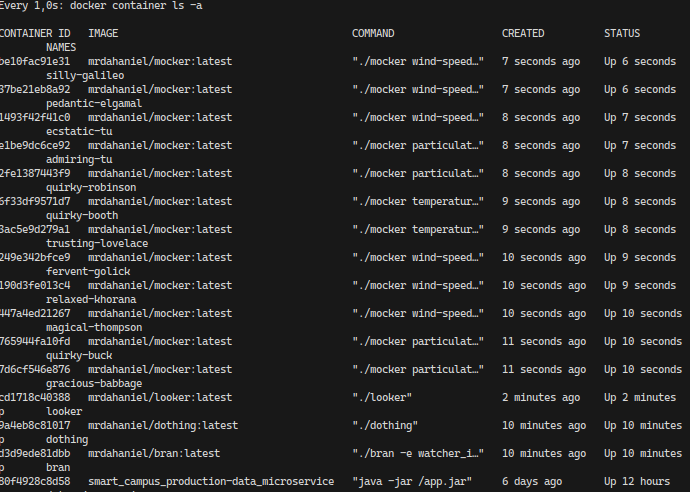
\includegraphics[width=0.9\linewidth]{images/ContainerLaunching.png}
    \vspace{-4mm}
\end{figure}

En total, se crearon 12 contenedores, que corresponden a los 12 componentes requeridos para el desarrollo de la aplicación. Cada uno de ellos configurado para suplir las necesidades de operación establecidas en el estado de referencia. Estos despliegues, como era de esperarse, fueron detectado por \textit{looker}, el cual realizó el nuevas valoraciones del estado. 

Los valores por defecto de los servicios usados para estas pruebas es un intervalo de tiempo entre mensajes de un minuto. Este valor por defecto, aunque para los requerimientos de datos cuyos \textit{timeout}, sean superiores, supliría las necesidades de la aplicación. Sin embargo, en el marco de esta simulación, esta frecuencia de reportes no es suficiente para cumplir con el estado de referencia de los requerimiento de temperatura de las locaciones.

Como consecuencia, el estado de la aplicación regresó a estado \textit{Fault}, y \textit{Bran}, al detectar los problemas, emitió las acciones tipo \textit{Restart} con el fin de traer los contenedores a un estado válido. Esto se puede ver en la figura \ref{fig:BranPlan2}.

\begin{figure}[H]
    \centering
    \caption{\\Bran identifica otros problemas en la aplicación}
    \label{fig:BranPlan2}
    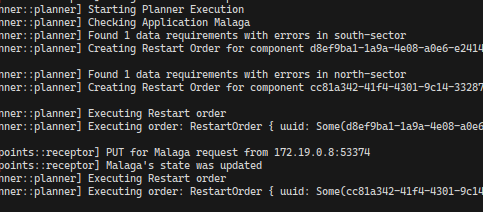
\includegraphics[width=0.9\linewidth]{images/BranRestarting.png}
    \vspace{-4mm}
\end{figure}

Este intento de reiniciar los servicios, como era de esperarse, no fue realmente efectiva debido a que la falla se debe a un problema en la configuración del servicio. Siendo así, la aplicación se mantuvo en estado de falla. Se esperaba que, ambos componentes encargados de la temperatura, al ya haber descartado el reinicio como un mecanismo efectivo para esta situación, fueran sometidos a una acción de reconfiguración, sin embargo, como se observa en la figura \ref{fig:BranPlan3}, en ese instante, sólo el componente de \texttt{north-sector} fue afectado.

\begin{figure}[ht]
    \centering
    \caption{\\Bran establece acciones de reconfiguración para adaptar la aplicación}
    \label{fig:BranPlan3}
    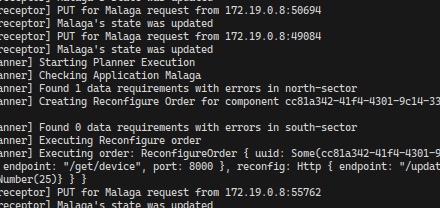
\includegraphics[width=0.9\linewidth]{images/BranReconfiguring.png}
    \vspace{-4mm}
\end{figure}

Esta reconfiguración fue ejecutada por \textit{DoThing}, y tomó efecto, alterando el valor por defecto entre mensajes, pasando de un reporte cada minuto, a uno cada 25 segundos\footnote{Según lo definido en las directivas presentes en el apéndice \ref{ape:DirectivesA}}. Con el nuevo valor, los componentes de temperatura, empezaban a reportar con mayor frecuencia, cumpliendo con las expectativas.

Poco tiempo después, el componente de temperatura de \texttt{south-sector}, reportó el estado de falla, por lo se ejecutó la misma acción de reconfiguración que con el componente de la otra locación, llevando el estado de la aplicación a \textit{Coherent}.

A partir de esta simulación, se pudo validar que el proceso implementado, tiene la capacidad de realizar la adaptación desde el peor escenario, hacia un esto de coherencia con la aplicación declarada inicialmente. Todas las acciones definidas por \textit{Bran}, permitieron modificar el estado de manera positiva.

Sin embargo, se identificaron algunas limitaciones de esta implementación. Como se observa en la figura \ref{fig:BranPlan3}, se muestra que \texttt{south-sector} no presenta problemas en sus requerimientos, cuando, debido a su configuración, debía estar en estado de falla. 

Esto se debe a un \textit{quirk} de la implementación realizada. Al manejar los procesos cada cierto intervalo de tiempo, es posible que un componente se encuentren en estado de falla, pero alcance a pasar a coherente justo antes de la evaluación de las acciones a tomar. Eventualmente, el componente fallaría en reportar antes de una una de las evaluaciones desencadenando en una acción, como fue el caso con la tardía reconfiguración del componente de \texttt{south-sector}. 
\subsection{Resultados De Escenario Experimental B}

El objetivo principal del escenario experimental B, era evaluar la capacidad de la implementación realizada de recuperar una aplicación en estado de coherencia, en donde se presenta una falla masiva, nuevamente a un estado válido; al igual que la capacidad de Bran de manejar más de una aplicación, como se había nombrado en la sección \ref{sec:Centering}.

Igual que durante el escenario experimental A, se realizó el despliegue de los servicios \textit{Bran} y \textit{DoThing}. Como se observa en la figura \ref{fig:Bran2Apps}, se definieron las arquitecturas objetivo de las dos aplicaciones a monitorear, al igual que las directivas a usar durante este proceso.

\begin{figure}[ht]
    \centering
    \caption{\\Aplicaciones y directivas registradas en Bran}
    \label{fig:Bran2Apps}
    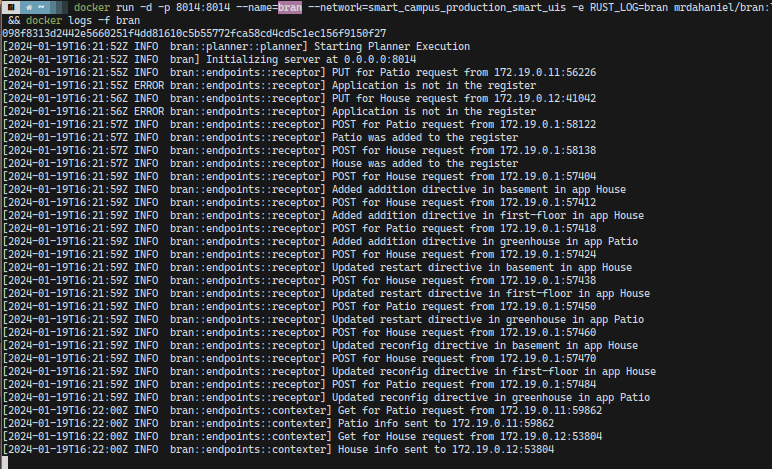
\includegraphics[width=0.9\linewidth]{images/BranBScenarioDeclarition.png}
    \vspace{-4mm}
\end{figure}

Seguidamente, como se observa en la figura \ref{fig:Looker2Apps}, se desplegaron los servicios de \textit{Looker} para cada una de las aplicaciones a monitorear. Ya con esta base lista, y como se definió en los pasos a seguir, se desplegaron de manera manual, un total de 3 servicios \textit{Mocker} con configuraciones específicas (tanto de los datos que estos reportaban, como de los tiempos de reporte) con el fin de cumplir con los requerimientos de datos definidos para las dos aplicaciones. 

\begin{figure}[H]
    \centering
    \caption{\\Dos instancias de looker monitoreando las aplicaciones declaradas}
    \label{fig:Looker2Apps}
    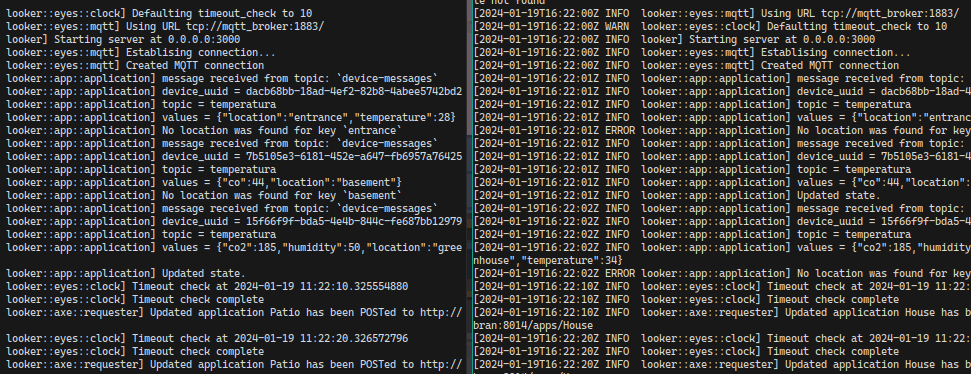
\includegraphics[width=0.9\linewidth]{images/Looker2Apps.png}
    \vspace{-4mm}
\end{figure}

Como era de esperarse, con las configuraciones hechas a la medida de las aplicaciones, el estado de estas era \textit{Coherent}, sin la necesidad de ningún tipo de cambios en los dispositivos. Siendo así, como se ve en la figura \ref{fig:KillThemAll}, se matan los 3 contenedores desplegados, y se elimina uno de ellos.

\begin{figure}[H]
    \centering
    \caption{\\Se matan los contenedores con los servicios iniciales}
    \label{fig:KillThemAll}
    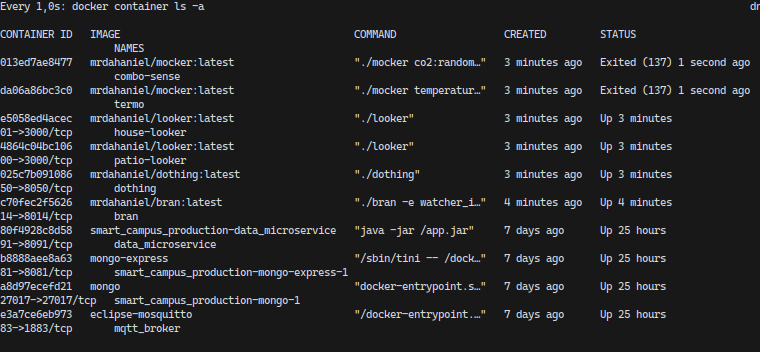
\includegraphics[width=0.9\linewidth]{images/Killing.png}
    \vspace{-4mm}
\end{figure}

La figura \ref{fig:FindAny}, muestra el como \textit{Bran}, define las órdenes para reiniciar los servicios para traer la aplicación a un estado nuevamente. En condiciones normales, se esperaría que esto sea lo único a realizar para adaptar la arquitectura, sin embargo, este no fue el caso.

\begin{figure}[ht]
    \centering
    \caption{\\Bran intenta reiniciar los contenedores}
    \label{fig:FindAny}
    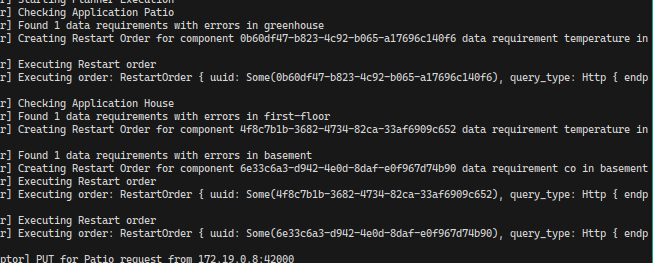
\includegraphics[width=0.9\linewidth]{images/BranOrdersRestarts.png}
    \vspace{-4mm}
\end{figure}

\newpage

Ya que los contenedores no fueron desplegados, o ha sido modificados, de ninguna manera por \textit{DoThing}, no estos no están mapeados. Siendo así, como se ve en la figura \ref{fig:CantFindAny}, es necesario buscar los contenedores en la red, pero, al estar los servicios muertos, y depender de la consulta \textit{Http} para poder identificarlos, no puede encontrarlos.


\begin{figure}[ht]
    \centering
    \caption{\\DoThing no puede encontrar los contenedores}
    \label{fig:CantFindAny}
    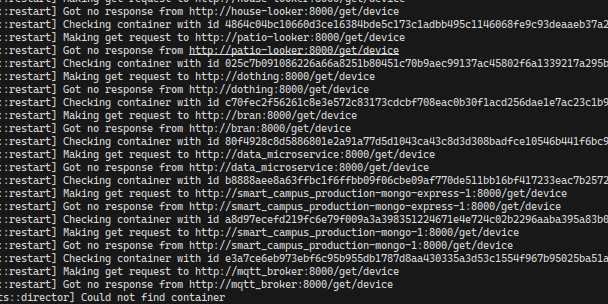
\includegraphics[width=0.9\linewidth]{images/CantFind.png}
    \vspace{-4mm}
\end{figure}

Esto demuestra otra de las falencias con la implementación realizada, que es la búsqueda del crecimiento de la fase de conocimiento. El haber identificado los componentes, antes de que se presentaran problemas, hubiera posibilitado la ejecución de órdenes cuando los servicios estén caídos. Así mismo, se hubiera podido establecer una búsqueda que no dependiera del estado de los componentes, quizás usando tags.

El resultado final, es que \textit{Bran}, al no poder actuar de otra manera, como se observa en la figura \ref{fig:HadToAdd}, ordena acciones de adición para suplir los componentes. Esto, eventualmente, resulta en el regreso de la aplicación a un estado válido, pero sigue sin ser lo ideal.

\begin{figure}[ht]
    \centering
    \caption{\\Bran crea órdenes de adicción}
    \label{fig:HadToAdd}
    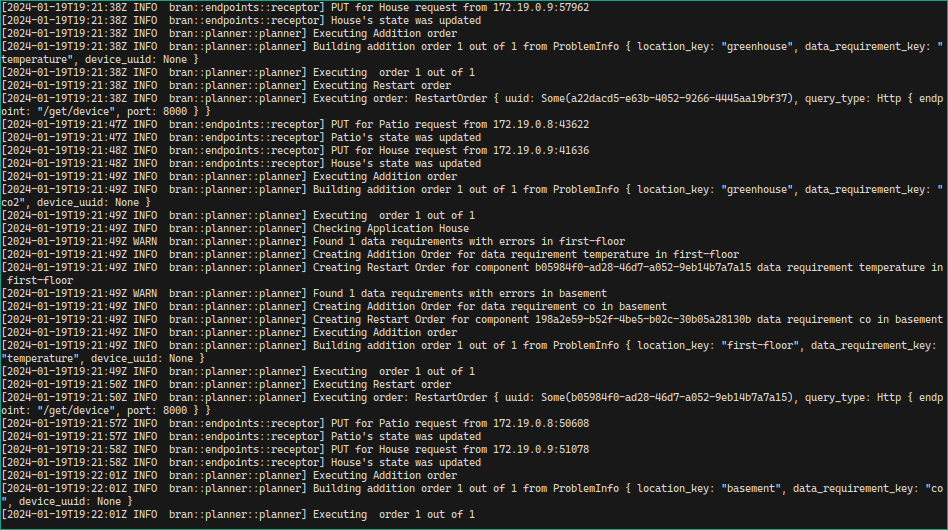
\includegraphics[width=0.9\linewidth]{images/ReLaunchIT.png}
    \vspace{-4mm}
\end{figure}


    \newpage
\section{\ Conclusiones y Trabajo Futuro} \label{sec:future}

El presente trabajo buscaba realizar la implementación de mecanismos de adaptación de arquitecturas a la plataforma Smart Campus UIS, que permitiera alterar el estado de una aplicación hacia un estado de referencia, de manera autonómica.

Para ello, se desarrolló e implementó un metamodelo capaz representar dichas arquitecturas, al igual que una manera de declararla tomando como foco los datos requeridos para su correcto funcionamiento; el cual cumple con el objetivo de establecer un estado de referencia.

También se diseño, e implementó, un servicio capaz de interpretar los mensajes de los dispositivos y evaluar el estado de la aplicación; al igual que una proceso de identificar los problemas y definir las acciones a tomar; cumpliendo con el objetivo de determinar una manera por la cual se pudieran realizar dichas comparaciones.

Así mismo, se diseñaron mecanismos que dieran la capacidad de modificar la arquitectura, hacia el estado de referencia definido; cumpliendo con el objetivo de reducir la cantidad de diferencias entre el estado observado, y el deseado.

Finalmente, se validaron las implementaciones realizadas, al igual que se identificaron las falencias de las mismas, dando paso a un nuevo foco de trabajo, ajustando, afinando y extendiendo las maneras en las que se pueden adaptar las arquitecturas de manera autonómica, al igual que estandarizando y simplificando la manera en la que se trabajan con estas herramientas.

De esta primera implementación, rara vez se sale de una línea de comando, por lo que el desarrollo de interfases para los diversos servicios implementados, con el fin de facilitar la accesibilidad a la plataforma.

Así mismo, la extensión de manera de evaluar los estados del sistema, a partir de diferentes datos definidos por el usuario, como uso de promedios para flexibilizar las fallas o contadores, antes de tomar acciones para ignorar fallos temporales, son puntos importantes a mejorar en futuras versiones.

También se ha de considerar la reimplementación de algunos de los mecanismos, con el fin de aumentar su eficacia en modificar los estados. Al igual que la expansión de la base de conocimiento, con el fin de aprovechar todos los recursos disponibles, independiente del estado de algunos componentes.

Se recomienda el buscar formas de permitir, al usuario, definir procesamientos de datos extra para la evaluación de el estado de referencia. Idealmente de manera agnóstica al lenguaje de programación usado. Lo cual daría un valor extra a la flexibilidad de la plataforma.

Finalmente, se recomienda la realización de pruebas más extensas, con dispositivos no simulados, que permitan evolucionar este primer prototipo de plugin para Smart Campus UIS, a algo que se pueda desplegar con relativa facilidad, independientemente del la aplicación que se esté desarrollando.

% 1. Implementar Lexical como algo más gráfico, 
% 2. Looker custom comparators
% 3. Live Update the desired state
    
    \newpage
    % \pagenumbering{Alph}
    \bibliography{bibliography.bib}
    
    % \appendix
    \begin{appendices}
        % \appendix
        % \newpage
        \section*{Apéndices}
        
\subsection{Directivas declaradas la aplicación Malaga} \label{ape:ExpA}

\lstinputlisting[language=YAML]{metamodel/model scenario A.yaml}


\newpage

\subsection{Directivas de la aplicación Malaga} \label{ape:DirectivesA}

\small
\linespread{0}
\lstinputlisting[language=Json]{metamodel/malaga-directives.json}


\newpage

\subsection{YAML de la aplicación Patio} \label{ape:ExpB1}

\lstinputlisting[language=YAML]{metamodel/model B1.yml}


\vspace{1cm}

\subsection{YAML la aplicación House} \label{ape:ExpB2}

\lstinputlisting[language=YAML]{metamodel/model B2.yml}


\newpage

\subsection{Directivas de la aplicación Patio} \label{ape:directivesB1}

\lstinputlisting[language=json]{metamodel/directivesB1.json}


\newpage

\subsection{Directivas de la aplicación House} \label{ape:directivesB2}

\lstinputlisting[language=json]{metamodel/directivesB2.json}


\newpage

    
    \end{appendices}


    % \include{sections/9. Apendices/metamodel}

\end{document}
